\documentclass[11pt,twoside,a4paper,titlepage]{article}
%\usepackage{csvsimple}  Denne giver fejl "\trimspace already defined"
\usepackage{amsmath}
\usepackage{amssymb}
\usepackage[nottoc, numbib, notlot, notlof]{tocbibind}
\usepackage{fancyhdr}
\usepackage{graphicx}
\usepackage[utf8]{inputenc} 
\usepackage{lastpage}
\usepackage[margin=2.5cm]{geometry}
\usepackage{mathtools}
\usepackage[danish]{babel}
\usepackage[svgnames]{xcolor}
\usepackage{newclude}
\usepackage{siunitx}
\usepackage{booktabs}
\usepackage{caption}
\usepackage{subfig}
\usepackage{wrapfig} 
\usepackage[subfigure]{tocloft}
\usepackage{todonotes}
\usepackage{lastpage} 
\usepackage{lipsum,lastpage}  
\usepackage{hanging}
\usepackage{tabularx}
\setlength{\headheight}{15pt}
\usepackage{filecontents}
\reversemarginpar
%\bibliographystyle{plain}

\usetikzlibrary{positioning} % in the preamble
\usetikzlibrary{decorations.pathreplacing}
\usetikzlibrary{arrows,shapes}
\usepackage{longtable}
\usepackage{footnote}
%\usepackage{tablefootnote}




\usepackage{tikz-timing}
\usepackage{graphics}
\usepackage{siunitx}
\usepackage{tikz}
\usetikzlibrary{shapes,arrows,chains, scopes}
\usepackage{pgfplots}               
%\pgfplotsset{compat=1.8}           Ikke i brug
\usepackage[%
  europeanvoltages,
  europeancurrents,
  europeanresistors,
  americaninductors,
  smartlabels]{circuitikz}


\setcounter{tocdepth}{3} % Antal lag i indholdsfortegenlse.

\AtBeginDocument{\addtocontents{toc}{\protect\thispagestyle{empty}}} 
\AtBeginDocument{\addtocontents{lof}{\protect\thispagestyle{empty}}} 
\AtBeginDocument{\addtocontents{lot}{\protect\thispagestyle{empty}}} 
%\pagestyle{empty}

% caption størrelse
\captionsetup{font=footnotesize}

\usepackage{pdfpages}
\usepackage[pdftex,
 hyperfigures=true,
 pdfauthor={Forfattere},
 pdftitle={},
 pdfsubject={},
 pdfkeywords={},
 hidelinks,
 plainpages=false,
 pdfpagelabels,
 unicode]{hyperref}
 

\newenvironment{changemargin}[2]{%
\begin{list}{}{%
\setlength{\topsep}{0pt}%
\setlength{\leftmargin}{#1}%
\setlength{\rightmargin}{#2}%
\setlength{\listparindent}{\parindent}%
\setlength{\itemindent}{\parindent}%
\setlength{\parsep}{\parskip}%
}%
\item[]}{\end{list}}

\setcounter{secnumdepth}{5}


%tegne figurer

\usepackage{graphicx} % den skal bruges til MATLAB figurer og formatet er: .eps
\usepackage{mathtools}

\usepackage{tikz-timing}
\usepackage{graphics}
\usepackage{siunitx}
\usepackage{tikz}
\usetikzlibrary{shapes,arrows,chains, scopes}







%% kode

\usepackage{listings}
\usepackage{color}

\definecolor{dkgreen}{rgb}{0,0.6,0}
\definecolor{gray}{rgb}{0.5,0.5,0.5}
\definecolor{mauve}{rgb}{0.58,0,0.82}

\lstset{frame=tb,
tabsize=4,
  language=C++,
  captionpos=b,
  tabsize=3,
  frame=false,
  numbers=left,
  numberstyle=\tiny,
  numbersep=5pt,
  breaklines=true,
  showstringspaces=false,
  basicstyle=\ttfamily,
%  identifierstyle=\color{magenta},
  keywordstyle=\color[rgb]{0,0,1},
   commentstyle=\color{ForestGreen}\ttfamily,
                morecomment=[l][\color{magenta}]{\#},
  stringstyle=\color{red}
}




\input{./content/task_diagram_styles_v2}
\input{./content/controller_diagram_styles_v1}
\begin{document}
\pagenumbering{Roman}
\title{POLE POSITION \\ DAT2, Robotteknologi 2. semesterprojekt}
\author{Gruppe 1 \\ Mikael, Mikkel, Nikolaj, Lars \& Anders}
\date{Maj 2013}
\begin{figure}
\centering
\includegraphics[width=1\textwidth]{graphics/forside.png}
\end{figure}
\maketitle




%\cleardoublepage
\clearpage
\section*{Abstract}

\todo[inline,author=ALLE]{Mangler at blive skrevet}
\include{./content/templates} % Kan bruges til copy paste ind i rapport for forskellige outputs.....




\vspace{3cm}
{
\newcommand{\namesigdate}[2][5cm]{%
  \begin{tabular}{@{}p{#1}@{}}
    #2 \\[2\normalbaselineskip] \hrule \\[0pt]
%    {\small \textit{Signature}}% \\[2\normalbaselineskip] \hrule %\\[0pt]
    %{\small \textit{Date}}
  \end{tabular}
}
\begin{changemargin}{-0cm}{-0cm}
\centering
\noindent \namesigdate[4.3cm]{Åse Videbæk Jensen} \hspace{1cm} \namesigdate[4.3cm]{Nikolaj Iversen} \hspace{1cm} \namesigdate[4.3cm]{Mikkel Jaedicke} \\~\\~\\
\centering
\noindent \namesigdate[4.3cm]{Anders Launer Bæk} \hspace{1cm}  \namesigdate[4.3cm]{Mikael Westermann} \hspace{1cm}   \namesigdate[4.3cm]{Michael Kjær Schmidt}
\end{changemargin}
}
\bigskip
\section*{Ansvarsområder}
De primære ansvarsområder er listet i nedenstående tabel
\bigskip
\begin{table}[!th]
\centering
\setlength{\extrarowheight}{5pt}
 \begin{tabular}{r|l}
Navn&Opgaver/Ansvarsområder \\[6pt] \hline
Åse&\\
&\\[6pt] \hline
Mikkel& DJ\\ 
& Food supply\\[6pt] \hline
Mikael&\\
&\\[6pt] \hline
Nikolaj&\\
&\\[6pt] \hline
Anders&\\
&\\[6pt] \hline
Michael & \\
&\\ 
\end{tabular}     
\caption*{Viser fordelingen af ansvarsområder.}            
\end{table}\\~\\ 
Det skal understreges, at tabellen er vejledende og at hele gruppen har været med over alle områder.
\todo[inline,author=Mikael]{trololol skriv ansvarsområder}


\newpage



%\makeatletter
%\makeatother
\newlength\mylen
\renewcommand\thepart{\Roman{part}}
\renewcommand\cftpartpresnum{Part~}
\settowidth\mylen{\bfseries\cftpartpresnum\cftpartaftersnum}
\addtolength\cftpartnumwidth{\mylen}


\tableofcontents
\listoffigures
\listoftables  

\subsection*{Indhold CDROM}
\begin{figure}[th!]
\centering
\begin{tabular}{l|l}
Hvad&Sti\\\hline
Rapporten&/Master\_doc.pdf\\
&/Data/\\
&/PIDoptimering/\\

\end{tabular}
\captionsetup{type=table}
%\caption[Indhold på CDROM'en]{Ovenstående tabel beskriver indholdet på CDROM'en.}
\label{tb:CD}
\end{figure}
\todo[inline,author=Mikael]{Indhold på CD-ROM'en}
\todo[inline, color=pink, author = Mikkel]{Ændr' Parts -  det er ikke dansk. Kunne ikke selv finde ud af det.}






\newpage
\subsection*{Tekst som mangler at blive skrevet}
\listoftodos
\pagestyle{fancy}
\fancyfoot{}
\fancyfoot[LE,RO]{\thepage}
\fancyfoot[LO,CE]{}
\fancyfoot[CO,RE]{}

% Disable indentation
\setlength{\parindent}{0pt}
\setlength{\parskip}{0.7\baselineskip}%




\section*{Forkortelser}

ES = English Skeet \\
PTS = Pan and Tilt System

\subsection*{Huske liste}
\begin{itemize}
\item Tallene skal stå kommaspereret.
\item \todo[inline,author=Anders]{Mikael, vil du ikke lige tjekke op det der står i sec:4. Jeg er i tvivl om B. Jeg har kigget andre steder, hvor der står vi skal bruge den viskøse friktion og ikke kb eller kt.}
\end{itemize}



\subsection*{Mangler at blive laver/skrevet}
\begin{itemize}
\item Abstract
\item Forord
\item Indledning
\item Pan \& Tilt-rammernes inertimoment
\item Reguleringsdesign
\item FPGA (Første udkast er lavet)
\item Mikrokontroller
\item Kommunikation mellem FPGA og Mikrokontroller
\item 
\listoftodos

\end{itemize}
\section*{Forord}
Projektet er udarbejdet som en del af 4. semester kurset ”Indlejrede systemer”, under bachelordelen af Civilingeniøruddannelsen i Robotteknologi. 
Projektet blev udarbejdet i tidsrummet 19. februar til 28. maj 2014, af en gruppe på 6 studerende.
Rapporten beskriver udarbejdelsen af lerduetracking på et Pan & Tilt system. 
Herunder lægges især vægt på hvilke valg der er truffet undervejs og hvorfor. 
Rapportens målgruppe er andre studerende med kompetenceniveau svarende til 4. semester eller derover, på samme eller lignende uddannelser.
Formålet med projektet er at kombinere semestrets forskellige fagligheder, og samtidig oparbejde kompetencer i problemorienteret projektarbejde.





%Nedenstående er Egon Olsen citat.
%~\\[1 cm]
%\textit{Må jeg være fri! Ti stille! Det er for galt. Jeg finder mig ikke i det! Det er det samme hver gang. Det er det samme hver eneste gang. Man har en plan - en genial plan! - og så er man omgivet af hundehoveder og hængerøve, lusede amatører, elendige klamphuggere, latterlige skidesprællere, talentløse skiderikker, impotente grødbønder, småbørnspædagoger og socialdemokrater!}
%\\[1 cm]
%\textit{\textbf{-Egon Olsen}}
\section{Indledning}
\citep[Side. 2]{reflist}
%%%%%%%%% RAPPORTENS KAPTILER BEGYNDER!!!
%\thispagestyle{empty}
\cleardoublepage
\pagenumbering{arabic}
\setcounter{page}{1}
\part{Applikation}
Nedenstående sektioner gennemgår de grundlæggende udgangspunkter for projektet.  

\section{Problemformulering}
Tracking af en lerdue i English Skeet (ES) vha. Pan and Tilt System (PTS). 
Lerduens position bestemmes som funktion af tiden, hvor specifikationerne for lerduens flugt er givet ved reglerne for ES, \citep{ES_regler}.

\begin{figure}[th!]
\centering
\includegraphics[width=1\textwidth]{./graphics/skeet_diagram_cropped_axes}
\caption[tekst i indholdsfortegnelsen]{figurtekst}
\label{fig:ES}
\end{figure}	
Systemets input er 60 kartesiske koordinatsæt (x ; y ; z) per sekund. Hvor de kartesiske koordinater kommer fra er uden for projektafgrænsningen. \\

I ES affyres serier af lerduer fra "High House" eller "Low House". Gennem serien skifter skytten mellem de otte stationer langs cirkelperiferien. Det kartesiske koordinatsystems origo ses på skitsen over banen, figur \ref{fig:ES}.\\

Det kartesiske koordinatsystem har origo på banens centrum. Akserne er indtegnet på figur \ref{fig:ES}. PTS's origo er placeret 45 [cm] over jorden. PTS står i udgangsposition med \(\phi\) og \(\theta\) lig med 0. Dvs. at tilts ramme står parallelt med yz-planet og det påmonteret gevær er parallelt med x-planet.\\

Geværet der bruges i ES har en spredning på ca. 2\degree. Systemet skal altså sigte efter målet med en nøjagtighed på \(\pm 1 \degree\) før geværet affyres. Ideelt set skal skytten skyde ca. når lerduen rammer toppunktet. Derfor skal PTS følge være "settlet" på lerduen inden lerduens toppunkt er nået.\\

Pans rotationen er begrænset til 170\degree\todo[author=Michael]{Mangler: Mål pan-rammens bevægelsesfrihed} omkring z-planet. Dette begrænser derved PTS maksimale overshoot.\\

Lerduen bliver affyret med en hastighed på 34,589 \([\frac{m}{s}]\) i en vinkel på \(9,103^{\circ}\) ift. xz-planet, i 3D-rummet med negligerbar luftmodstand og tyngdekraft. Set ovenfra bevæger målet sig som set på figur \ref{fig:para_in_xy_plane}. 
På figur \ref{fig:HH2D_para} ses nedslagspunktet, G, fra High-House 52 [m] efter startpositionen, D, samt  
PTS placering i punktet B.\\
\begin{figure}[h!]
\centering
\subfloat[Lerduens højde som funktion af afstanden.\label{fig:HH2D_para}]{%
	\begin{tikzpicture}[scale=0.8]
	\include*{./graphics/high_house_2D_parabola}
	\end{tikzpicture}
}
\subfloat[Lerduens bane projekteret på xy-planet.\label{fig:para_in_xy_plane}]{%
	\begin{tikzpicture}[scale=0.16]
	\include*{./graphics/parabola_in_xy_plane}
	\end{tikzpicture}
}
\caption[Lerduens parabel i 2D]{Viser parablen af lerduens bane i 2D.}
\end{figure}

PTS dimensioneres til en konkurrence i ES og er afgrænset til et enkelt tilfælde: Afskydning fra ”High-House” med PTS placeret på station 4. Øvrige kravspecificeringer fåes i sektion \ref{sec:kravspecifikation}.
\section{Kravspecifikation}
\label{sec:kravspecifikation}
Kravene til systemet findes vha. reglerne for English Skeet \citep{ES_regler}.
%samt det udleverede systems fysiske begrænsninger.

Lerduens bane beregnes vha. de i reglerne givne værdier for affyringspunkt (D), forventet nedslagspunkt (G)
og "target crossing point" (TCS).
%Med antagelsen om negligerbar luftmodstand kan en kasteparabel således udregnes ved interpolation af disse tre punkter.
Lerduens parabel findes ved interpolation af disse tre punkter. Det antages at luftmodstanden er negligerbar.
%Kasteparablen er givet ved ligning \ref{eq:ks:vektorparabel3d}, med origo som angivet på figur \ref{fig:ES}.
%\begin{equation}
%Pos\left( t \right) = 
%\left( \begin{matrix} 
%	x\left( t \right)  \\ 
%	y\left( t \right)  \\ 
%	z\left( t \right)  \end{matrix} \right) =
%	 \left( \begin{matrix} 
%	- 9,34\cdot t+5,5 \\
%  32,851\cdot t-19,3 \\ 
% -{ 4,91\cdot t }^{ 2 }+5,473\cdot t+3,05\end{matrix} \right) [\text{m}]
%\label{eq:ks:vektorparabel3d}
%\end{equation}

%Med kasteparablen er det muligt at specificere systemets betingelser yderligere:
%Lerduens affyringshastighed og vinkel ift. xy planet kan lerduens flugt beregnes. 
%
Lerduens affyringshastighed og vinkel ift. xy planet blev beregnet vha. den fundne kasteparabel. 
Lerduen affyres med en hastighed på 34,589 \([\frac{m}{s}]\) i en vinkel på \(9,103 \degree\) 
ift. xy-planet jf. figur \ref{fig:ES}\footnote{Beregningerne bag kasteparablen findes i appendix \ref{sec:udregning_af_parabel}.}. 

Lerduens flugt er givet i ligning \ref{eq:ks:vektorparabel3d} med origo som angivet på figur \ref{fig:ES}. 

\begin{equation}
Pos\left( t \right) = 
\left( \begin{matrix} 
	x\left( t \right)  \\ 
	y\left( t \right)  \\ 
	z\left( t \right)  \end{matrix} \right) =
	 \left( \begin{matrix} 
	- 9,34\cdot t+5,5 \\
  32,851\cdot t-19,3 \\ 
 -{ 4,91\cdot t }^{ 2 }+5,473\cdot t+3,05\end{matrix} \right) [\text{m}]
\label{eq:ks:vektorparabel3d}
\end{equation}
%En gennemgang af beregningerne der ligger bag kasteparablen findes i appendix \ref{sec:udregning_af_parabel}.

Lerduens flugt er illustreret på figur \ref{fig:para_total}.
Punktet D er "high house".
Punktet SB og punktet G er hhv. 40,3 [m] og 52 [m] fra "high house". \\
\begin{figure}[h!]
\centering
\subfloat[Lerduens højde som funktion af afstanden til D.\label{fig:HH2D_para}]{%
	\begin{tikzpicture}[scale=0.8]
	\include*{./graphics/high_house_2D_parabola}
	\end{tikzpicture}
}
\subfloat[Lerduens bane projekteret på xy-planet.\label{fig:para_in_xy_plane}]{%
	\begin{tikzpicture}[scale=0.16]
	\include*{./graphics/parabola_in_xy_plane}
	\end{tikzpicture}
}
\caption[Lerduens parabel i 2D]{Viser parablen som udgør lerduens bane i 2D.}
\label{fig:para_total}
\end{figure}

Tilt-rammen kan bevæge sig frit,
men pan-rammen kan pga. en stopklods kun rotere \(154 \degree\)\footnote{Målt eksperimentielt.}.

Haglene fra et 12 gauge haglgevær med Skeet Choke spredes så de dækker et område
%med en diameter på 1,32 [m] på en afstand til centrum af cirklen på 37 [m] 
med en diameter på 1,32 [m] på 37 meters afstand
\citep[Pattern and choke]{patternandchoke}.
Spredningsvinklen er, med en antagelse om lineær spredning, givet ved ligning \ref{eq:ks:spredning}.
\begin{align}
\begin{split}
  Spredning &= 2\cdot{}\tan^{-1}\left(\frac{1,32/2}{37}\right) \\
  &= 2,04 \degree
  \end{split}
  \label{eq:ks:spredning}
\end{align}
%Der er altså et krav om at geværet peger på lerduen med en præcision på \(\pm 1,02 \degree\).
Når tracking fejlen defineres ud fra pan-vinklen \(\theta\) og tilt-vinklen \(\phi\) som i ligning \ref{eq:ks:trackingerror} rammes 
lerduen ved afskydning af haglgeværet når ligning \ref{eq:trackingerrorkrav} opfyldes.
\begin{align}
  TE = \left | \begin{pmatrix}  \theta_{\text{target}}\\ \phi_{\text{target}}\end{pmatrix} - \begin{pmatrix} \theta_{current}\\ 
  \phi_{current}\end{pmatrix} \right | &&\text{(Tracking fejl)}
\label{eq:ks:trackingerror}
\\
	TE\leq 1,02 \degree && \text{(Lerduen rammes)}
\label{eq:trackingerrorkrav}
\end{align}

Settling Time defineres som tiden der går før tracking fejlen forbliver \(\leq 1.02 \degree\).
%som skrevet i ligning \ref{eq:ks:settlingtime}.
%\begin{align}
%{ { t }_{ s }\quad =\left t \right|  }_{ TE\leq 1,02 \degree }
%\label{eq:ks:settlingtime}
%\end{align}

Der affyres mellem det tidspunkt lerduen når toppunktet og SB.
I dette tidsrum skal PTS sigte præcist på lerduen under opfyldelse af ligning \ref{eq:trackingerrorkrav} og dette 
stiller krav til Settling Time, \(t_s\), som skrevet i ligning \ref{eq:ks:settlingtime1}.
%Tidspunktet, hvor lerduen når sit toppunkt er altså samtidigt tid er altså det højeste settling time må være, ligning \ref{eq:ks:settlingtime1}

\begin{align}
  t_{top} &= 0,557\text{ [s]} &\text{(Toppunktet af parablen)}
  \label{eq:ks:toppunktstid}
  \\
   t_{SB} &= 1,18\text{ [s]} &\text{(SB)}
  \label{eq:ks:toppunktstid}
  \\
  t_{s} & \leq 0,557\text{ [s]} &\text{(Krav til Settling Time)}
  \label{eq:ks:settlingtime1}
\end{align}

%I dette tidsrum skal Pan \& Tilt-systemet sigte præcist på lerduen og kravet til 
%tracking error i ligning \ref{eq:ks:trackingerrorsize} skal overholdes.
%Der er altså et tidsmæssigt krav til reguleringen om en indsvingningstid (Settling Time) for systemet,
%der er lavere end tiden \(t_{s}\) angivet i ligning, \ref{eq:ks:settlingtime}.
%Dette krav gælder for både pan-rammens vinkel (\(\phi\)) og tilt-rammens vinkel (\(\theta\)).
%For en 1-radian reference giver dette altså en maksimal tracking error (SSE) på 1,78 \%.
%\todo[inline, author=Michael]{Den virkelige sammenhænge er mere kompleks: Hvis både pan \& tilt rammen peger 1\degree ved siden af, er den samlede afvigelse vel over 1,02\degree}
%\todo[inline, color = pink, author = Mikkel]{Hvad mening giver det at kigge på 1 radian reference og kan man virkelig kalde det SSE?}
Det eneste krav der stilles til systemet er altså et Settling Time krav.

%Dette giver altså en øvre og en nedre grænse for pan-rammens maksimale udsving,
%som afhænger af reguleringen
%- et for højt overshoot på pan-positionen kan give udsving, der ikke holder sig inden for grænserne.
%Hvis det antages, at vinklen \(0 \degree\) er lige midt imellem pan-rammens rotationsgrænser,
%så den kan rotere \(77 \degree\) til hver side, så er det maksimale overshoot for et 1-radians step-input
%givet ved \(34 \%\).
%\todo[inline, color = pink, author = Mikkel]{Hvad mening giver den 1 radian reference?}
%\todo[inline, author=Michael]{Indsæt evt. figur med overshoot begrænsninger?}



\section{Projektoverblik}
\label{sec:projektoverblik}
%Anders afsnit:
%\todo[inline,author=Anders]{Der må gerne gives feedback.. jeg synes selv jeg er lidt på bar bund med hvad der skal stå}
%Inden rapportens kommende afsnit introdukseres et kort overblik af projektets komponenter og hvordan de kommunikerer med hinanden.\\
%Som der ses på nedenstående figur \ref{fig:overview_openloop_PTS}, er de forskellige komponenter opdelt i forskellige farver.\\
%De grønne kasser repræsenterer mikrocontrolleren som vha. UART kommunikerer med brugeren. \\
%FPGA'en er repræsenteret vha. en lilla kasse som er bindeledet mellem mikrocontrolleren og de to DC motorer. 
%FPGA'en og mikrocontrolleren kommunikere sammen vha. SPI. FPGA'en genererer to PWM-signaler, som driver hhv. H-broen og motor for pan og H-broen og motor for tilt. DC motorene sender deres encoder feedback til FPGA'en.

%Mikkels:
Som fremgår af projektoplægget skal projektet opdeles som vist på 
figur \ref{fig:overview_openloop_PTS}. 
Det ligger altså udenfor dette projekt at bestemme den overordnede opdeling.
Projektoplægget stiller ydermere følgende krav til implementeringen:
\begin{itemize}
\itemsep1pt
  \item Regulatorerne skal implementeres på én microprocessor.
  \item Der skal benyttes SPI kommunikationen imellem microprocessoren og FPGA’en.
  \item FPGA’en skal styre PWM signalerne til motorerne.
  \item FPGA’en skal benyttes til at bestemmes motorernes position via encoderne.
\end{itemize}

\bigskip

\begin{figure}[!th]
\centering
\begin{tikzpicture}[auto, node distance=1cm,>=latex']
\include*{./graphics/PTSoverview}
\end{tikzpicture}
\caption[Principskitse af PTS]{Principskitse af PTS med farvekoder.}
\label{fig:overview_openloop_PTS}
\end{figure}
\part{System identifikation}
\todo[color=green! 100,inline,author=ALLE]{SOME INTRO}

%\section{Matematisk model af Pan \& Tilt-systemet}
\section{Matematisk model af PTS}
\label{sec:matPTS}
Under designet af en regulator skal systemet identificeres. Der er forskellige metoder til systemidentifikation.
Én metode ser som udgangspunkt systemet som en "black box", og identificerer systemet
på baggrund af sammenhørende værdier for input og output.
En anden metode tager udgangspunkt i matematisk at beskrive de enkelte dele i systemet
for på den måde at sammenstykke en model af hele systemet.
Det vælges hovedsageligt at benytte den sidstnævnte metode til bestemmelsen af en simplificeret
model af Pan \& Tilt-systemet af følgende årsager:
\begin{itemize}
\itemsep1pt
\item Matematiske modeller for systemets enkelte elementer findes i litteraturen.
\item Flere af de matematiske modeller er lineære og simple.
\item De matematiske modeller giver indsigt i den involverede fysik og giver mulighed
	for at udtrykke systemets parametre i fysiske størrelser.
\end{itemize}
Ulempen ved at bruge teoretiske \textit{lineære} matematiske modeller er,
at de altid vil være tilnærmelser, og ikke beskriver ulineariteter som dødbånd og tidsforsinkelser.

%En skitse af Pan \& Tilt-systemet findes i figur \ref{fig:overview_openloop_PTS}.
%
\subsection{Afkobling af pan og tilt}
Når den ene af de to rammer roterer vil en kraftmoment-induceret præcession påvirke den anden ramme.
Samtidig vil tilt-rammens vinkel påvirke inertimomentet omkring pan-aksen, og dermed
pan-motorens overførselsfunktion.
Der er altså tale om et Multi-Input Multi-Output (MIMO) system med en kobling mellem pan og tilt.
Det vælges at simplificere systemet til to Single-Input Single-Output (SISO) systemer, som gruppen er bekendt med.
Retfærdiggørelsen heraf ligger i, at præcessionens størrelse afhænger af vinkelaccelerationen, som er stærkt begrænset
for dette fysiske system, samt at tilt-rammens inertimoment er tilnærmelsesvis konstant, som yderligere beskrevet i afsnit \ref{sec:inertimoment}.
Afkoblingen af de to systemer, og opdelingen i hhv. pan og tilt gør, at der kan udvikles en separat regulator
til hvert system, og at der skal findes en overførselsfunktion for hvert system.
De følgende beregninger tager altså udgangspunkt i det simplificerede afkoblede system.
Det er dog stadig vigtigt iht. kravspecifikationen at betragte tracking fejlen som en størrelse der samlet
ikke må overstige 1,02\degree, og på dette punkt betragtes systemet stadig som en helhed.

\subsection{DC-Motor}
To DC-motorer af typen EMG30 \citep{emgmotor}, er forbundet til systemet.
Det antages, at motorerne kan beskrives ved samme matematiske model.
Den matematiske model af DC-motoren er beskrevet i appendix \ref{sec:dcmotor},
der også beskæftiger sig med den eksperimentelle bestemmelse af parametrene for en EMG30-motor
(det antages, at systemets to motorer har samme parametre).
Motoren kan beskrives ved ligning \ref{eq:matVm_transient3}, hvor konstanterne \(k_1\), \(k_2\) og \(k_3\)
er givet ved ligningerne \ref{eq:matkonstanter}. Der henvises til appendix \ref{sec:dcmotor}
for yderligere forklaring af modellen.
\begin{equation}
	V_m\left(t\right)=k_1\cdot{}\frac{\mathrm d^2}{\mathrm d t^2} \big(\omega\left(t\right) \big)
		+k_2\cdot{}\frac{\mathrm d}{\mathrm d t} \big(\omega\left(t\right) \big)
		+k_3\cdot{}\omega\left(t\right)
	\label{eq:matVm_transient3}
 \end{equation}
\begin{equation}
	k_1=\frac{L_m\cdot{}\left(J_L+J_m\right)}{K_t},
	k_2=\frac{R_m\cdot{}\left(J_L+J_m\right)+L_m\cdot{}B}{K_t},
	k_3=K_b+\frac{R_m\cdot{}B}{K_t},
	\label{eq:matkonstanter} 
 \end{equation}
\(L_m\) er motorens ækvivalente induktans, \(R_m\) dens resistans, \(J_m\) dens indre inertimoment,
\(K_t\) er kraftmomentproportionalitetskonstanten, \(K_b\) er proportionalitetskonstanten for den modelektromotoriske kraft,
mens \(B\) er den viskøse friktionskoefficient.
\begin{figure}[th!]
	\centering
	%%%\begin{tabular}{r|l|l}
%%%Parameter&Værdi&Enhed\\\hline
%%%\(R_m\)&\(5,215\)&\([\Omega]\)\\
%%%\(L_m\)&\(2,2\cdot{}10^{-3}\)&\(\text{[H]}\)\\
%%%\(K_b\)&\(0,517\)&\(\left[ \frac{\text{V} \cdot \text{s} }{ \text{ rad } }  \right] \)\\
%%%\(K_t\)&\(0,517\)&\(\left[ \frac{\text{N}\cdot \text{m}}{\text{A}} \right] \)\\
%%%\(B\)&\(0,00319\)&\(\left[  \text{N} \cdot \text{m} \cdot \text{s}\right] \)\\
%%%\(J_m\)&\(8,26\cdot10^{-4}\)&\(\left[ \text{kg}\cdot{\text{m}^2} \right]  \)\\
%%%\item \(\left| T _f \right|\)&\(0,0571\)&\(\left[ \text{N} \cdot \text{m} \right]  \)\\
%%%\end{tabular}

\begin{tabu}{r|[1.25pt]l|l}
Parameter&Værdi&Enhed\\\tabucline[1.25pt]{-}
\(R_m\)&\(5,215\)&\([\Omega]\)\\
\(L_m\)&\(2,2\cdot{}10^{-3}\)&\(\text{[H]}\)\\
\(K_b\)&\(0,517\)&\(\left[ \frac{\text{V} \cdot \text{s} }{ \text{ rad } }  \right] \)\\
\(K_t\)&\(0,517\)&\(\left[ \frac{\text{N}\cdot \text{m}}{\text{A}} \right] \)\\
\(B\)&\(0,00319\)&\(\left[  \text{N} \cdot \text{m} \cdot \text{s}\right] \)\\
\(J_m\)&\(8,26\cdot10^{-4}\)&\(\left[ \text{kg}\cdot{\text{m}^2} \right]  \)\\
%\item \(\left| T _f \right|\)&\(0,0571\)&\(\left[ \text{N} \cdot \text{m} \right]  \)\\
\end{tabu}
	\captionsetup{type=table}
	\caption[Motorparametre]
			{Eksperimentelt bestemte motorparametre.}
	\label{tb:matmotorparametre}
\end{figure}
De eksperimentelt bestemte motorparametre står i tabel \ref{tb:matmotorparametre}.
Det er vigtigt at bemærke, at de to motorer adskiller sig fra hinanden ved parameteren \(J_L\), som er belastningens
inertimoment. Dette er ikke en egentlig motorparameter, men en parameter der udelukkende afhænger
af pan- og tilt-rammernes masser, dimensioner og vinkel.
Desuden er det værd at bemærke, at denne model ikke tager højde for statisk friktion og Coulomb-friktion,
fordi de ikke, som den viskøse friktion, er lineære. Ikke desto mindre antages det, at Coulomb-friktionen under
bevægelse giver en konstant dæmpning, der kan kompenseres for med en højere forstærkning.
%Anders: Jeg tænker ikke denne er nødtvendig..
%\todo[inline]{Skal vi bruge en kilde ang. Coulomb-friktion?}

Vi er interesserede i en overføringsfunktion for DC-motoren. Med antagelse om at \(\omega\) (vinkelhastigheden) og dens tidsafledte er 0
Laplace-transformeres ligning \ref{eq:matVm_transient3}, og den resulterende overføringsfunktion findes
i ligning \ref{eq:transOmega}.
\begin{equation}
	\frac{\Omega\left(s\right)}{V_m\left(s\right)}=\frac{1}{k_1\cdot{}s^2+k_2\cdot{}s+k_3}
	\label{eq:transOmega}
 \end{equation}
Ligning \ref{eq:transOmega} beskriver motorens rotors vinkelhastighed \(\Omega\left(s\right)\) som funktion af spændingsfaldet
\(V_m\left(s\right)\) over motoren. Bemærk at reduktionsgearingen i motoren gør at vinkelhastigheden af Pan \& Tilt rammerne
er lavere.
Vinkelhastigheden \(\omega\) er den tidsafledte af vinklen \(\theta\),
og hvis det antages at motorens startvinkel er 0, så kan motorens overføringsfunktion
findes ved tilføjelse af en integrator \(\frac{1}{s}\) til ligning \ref{eq:transOmega}.
Motorens overføringsfunktion \(G_m\left(s\right)\) fra input spændingsfald til output vinkel (inden reduktionsgearing) findes
i ligning \ref{eq:transTheta}.
\begin{equation}
	G_m\left(s\right)=\frac{\Omega\left(s\right)}{V_m\left(s\right)}\cdot{}\frac{1}{s}=\frac{1}{k_1\cdot{}s^3+k_2\cdot{}s^2+k_3\cdot{}s}
	\label{eq:transTheta}
\end{equation}
DC-motorens overføringsfunktion afhænger af dens belastning,
og belastningen (inertimomentet \(J_L\) der skal roteres) er indeholdt i konstanterne \(k_1\) og \(k_2\).
Der er altså en separat overføringsfunktion \(G_m\left(s\right)\) for Pan og for Tilt,
da rammerne har forskelligt inertimoment.
De to belastningsinertimomenter benævnes hhv. \(J_{pan}\) og \(J_{tilt}\),
og de to forskellige overføringsfunktioner benævnes hhv. \(G_{m,p}\) og \(G_{m,t}\).
Bestemmelsen af inertimomenterne findes i afsnit \ref{sec:inertimoment}.

\subsection{FPGA-modulerne}
\label{subsec:matFPGA}
FPGA'ens positionsencoders læser motorens vinkel inden reduktionsgearingen,
altså outputtet af \(G_m\left(s\right)\).
Der er altså tale om en kvantisering af output-vinklen.
Gearingen til rammerne er i forholdet 1:3, og da der er 360 encoder-ticks pr. rotation \citep{emgmotor},
er kvantiseringsintervallet \(\frac{1}{1080}\).

På FPGA'en genereres et PWM-signal til hver motors H-bro ud fra en
duty cycle som mikrocontrolleren leverer.
PWM-signalet forstærkes af H-broen til et firkantsignal med en amplitude på 12 [V],
som leveres til motoren.
En overføringsfunktion for denne duty cycle - motorspændingsfald konvertering ønskes
til reguleringen.
Det vælges at modellere konverteringen som en simpel lineær forstærkning af en duty cycle mellem -100 \% og +100 \%
til en DC-spænding mellem -12 [V] og +12 [V]. Med denne simple model ændres systemets orden ikke,
og det vurderes, at tidsforsinkelsen fra input duty cycle til motorbevægelse er negligerbar.
Overføringsfunktionen fra duty cycle til DC-spænding står i ligning \ref{eq:transPWM}.
\begin{equation}
	PWM\left(s\right)=PWM=12
	\label{eq:transPWM}
\end{equation}
\todo[inline,author=Mikael]{Dedikér et underafsnit til diskussion af tidsforsinkelser, digitale såvel som analoge.}
%\subsection{Pan \& Tilt-rammernes inertimoment}
\subsection{PTS's inertimoment}
\label{sec:inertimoment}
For at opnå den optimale respons, skal reguleringen tage højde for, at Pan \& Tilt-motorerne møder modstand i form af
Pan \& Tilt-rammernes inertimoment. Inertimomentet kan bestemmes ved kendskab til rammernes
masse og dimensioner. Beregningen tager udgangspunkt i den simplificerede model skitseret i figur \ref{fig:inerti_PTS}.
På figuren er rammernes enkelte længder markeret, og de er målt til \({L_{1}} =0,292\) [m],
\({L_{2}} =0,280\) [m], \({L_{3}}= 0,42\) [m], \({L_{4}} =0,246\) [m], \({L_{pro}}=0,04\) [m].
\begin{figure}[!th]
\centering
\begin{tikzpicture}[scale=0.8]
\include*{./graphics/inerti_PTS}
\end{tikzpicture}
\caption[Skitse af Pan \& Tilt-rammerne]{Skitse af Pan \& Tilt-rammerne.}
\label{fig:inerti_PTS}
\end{figure}

I appendix \ref{sec:inertimomentberegning} beregnes Tilt-rammens inertimoment omkring tilt-aksen,
Pan-rammens inertimoment omkring pan-aksen,
og Tilt-rammens påvirkning på inertimomentet omkring pan-aksen diskuteres.

Inertimomenterne er givet ved ligningerne \ref{eq:matinerti_tilt_pan_fak},
som beregnet i appendix \ref{sec:inertimomentberegning}.
\begin{align}
\label{eq:matinerti_tilt_pan_fak}
\begin{split}
{J_{tilt}}&=1,57499\cdot{10}^{-4} \text{ [kg m$^2$]}
\\
{J_{pan}}&=4,62172\cdot{10}^{-4} \text{ [kg m$^2$]}
\end{split}
\end{align}
\(J_{pan}\) er beregnet ud fra et konstant bidrag fra tilt-rammen under antagelsen om,
at denne står tilnærmelsesvis lodret under hele bevægelsen.

%\subsection{Pan- og tilt-systemernes åbensløjfeoverføringsfunktioner}
\subsection{PTS's åbensløjfeoverføringsfunktioner}
Hvert SISO-undersystem består af én PWM-blok på FPGA'en og en DC-motor med belastning.
To overføringsfunktioner \(G_{pan}\) og \(G_{tilt}\) for pan- og tilt-systemet kan opskrives
som produktet af ligning \ref{eq:transPWM} og \ref{eq:transTheta}. De to overføringsfunktioner
står i ligningerne \ref{eq:transpantilt0}, og de er illustreret i figur \ref{fig:openloop1}.
\begin{align}
\label{eq:transpantilt0}
\begin{split}
	G_{pan}\left(s\right)&=PWM\left(s\right)\cdot{}G_{m,p}\left(s\right)\\
	&=12\cdot{}\frac{1}
			{\left(\frac{L_m\cdot{}\left(J_{pan}+J_m\right)}{K_t}\right)\cdot{}s^3
			+\left(\frac{R_m\cdot{}\left(J_{pan}+J_m\right)+L_m\cdot{}B}{K_t}\right)\cdot{}s^2
			+\left(K_b+\frac{R_m\cdot{}B}{K_t}\right)\cdot{}s}\\
	&\approx\frac{2,24\cdot{}10^6}{s^3 + 2,43\cdot{}10^3 \cdot{} s^2 + 1,03\cdot{}10^5\cdot{}s}
	\\
	\\
	G_{tilt}\left(s\right)&=PWM\left(s\right)\cdot{}G_{m,t}\left(s\right)\\
	&=12\cdot{}\frac{1}
			{\left(\frac{L_m\cdot{}\left(J_{tilt}+J_m\right)}{K_t}\right)\cdot{}s^3
			+\left(\frac{R_m\cdot{}\left(J_{tilt}+J_m\right)+L_m\cdot{}B}{K_t}\right)\cdot{}s^2
			+\left(K_b+\frac{R_m\cdot{}B}{K_t}\right)\cdot{}s}\\
	&\approx\frac{2,93\cdot{}10^6}{s^3 + 2,43\cdot{}10^3 \cdot{} s^2 + 1,34\cdot{}10^5\cdot{}s}
\end{split}
\end{align}
\begin{figure}[!th]
\centering
\begin{tikzpicture}[auto, node distance=2.6cm,>=latex']
\include*{./graphics/openloop1}
\end{tikzpicture}
\caption[Åbensløjfeoverføringsfunktioner]{Åbensløjfeoverføringsfunktionerne \(G_{pan}\left(s\right)\) og \(G_{tilt}\left(s\right)\).
	Signalet \(d.c.\left(t\right)\) er en duty cycle mellem -100 \% og +100 \%.}
\label{fig:openloop1}
\end{figure}

Åbensløjfeoverføringsfunktionerne \(G_{pan}\) og \(G_{tilt}\) danner udgangspunktet
for analysen der hører til designet af reguleringssløjferne.
I afsnit \ref{subsec:verifikation} nedenfor diskuteres overføringsfunktionernes nøjagtighed,
og der gives forslag til forbedring af modellen ift. det fysiske system som det fungerer
i praksis.

\subsubsection{Verifikation}
\label{subsec:verifikation}
Åbensløjferesponsen af Tilt-systemet er blevet målt og sammenlignet med den teoretiske respons.
Grunden til, åbensløjferesponsen kun er blevet målt for Tilt er, at rammen kan rotere frit,
mens pan blokeres af en stopklods.
Sammenligningen er nødvendig for at verificere modellen, og for evt. at kunne justere modellen,
så udgangspunktet for analysen der hører til designet af reguleringssløjferne er så godt som muligt.

Der blev som input givet et rampesignal, der gik fra 0 \% duty cycle til næsten 100 \% duty cycle
i løbet af ca. 12 sekunder. Tilt-vinklen blev målt med FPGA'en og sammenlignet med den teoretiske
respons for samme input-signal.
Forsøget blev udført syv gange.

Den målte vinkel skal differentieres, således at integratoren i \(G_{tilt}\) ikke gør,
at fejlen i forhold til de målte data akkumuleres over tid.
Måden den målte vinkel er blevet differentieret på er ved først at fitte en parabel
til vinklen som funktion af tiden vha. Least Squares metoden. Herefter differentieres
parablen, og den resulterende rette linje er altså et mål for vinkelhastigheden som funktion af tiden.

\begin{figure}[th!]
	\centering
	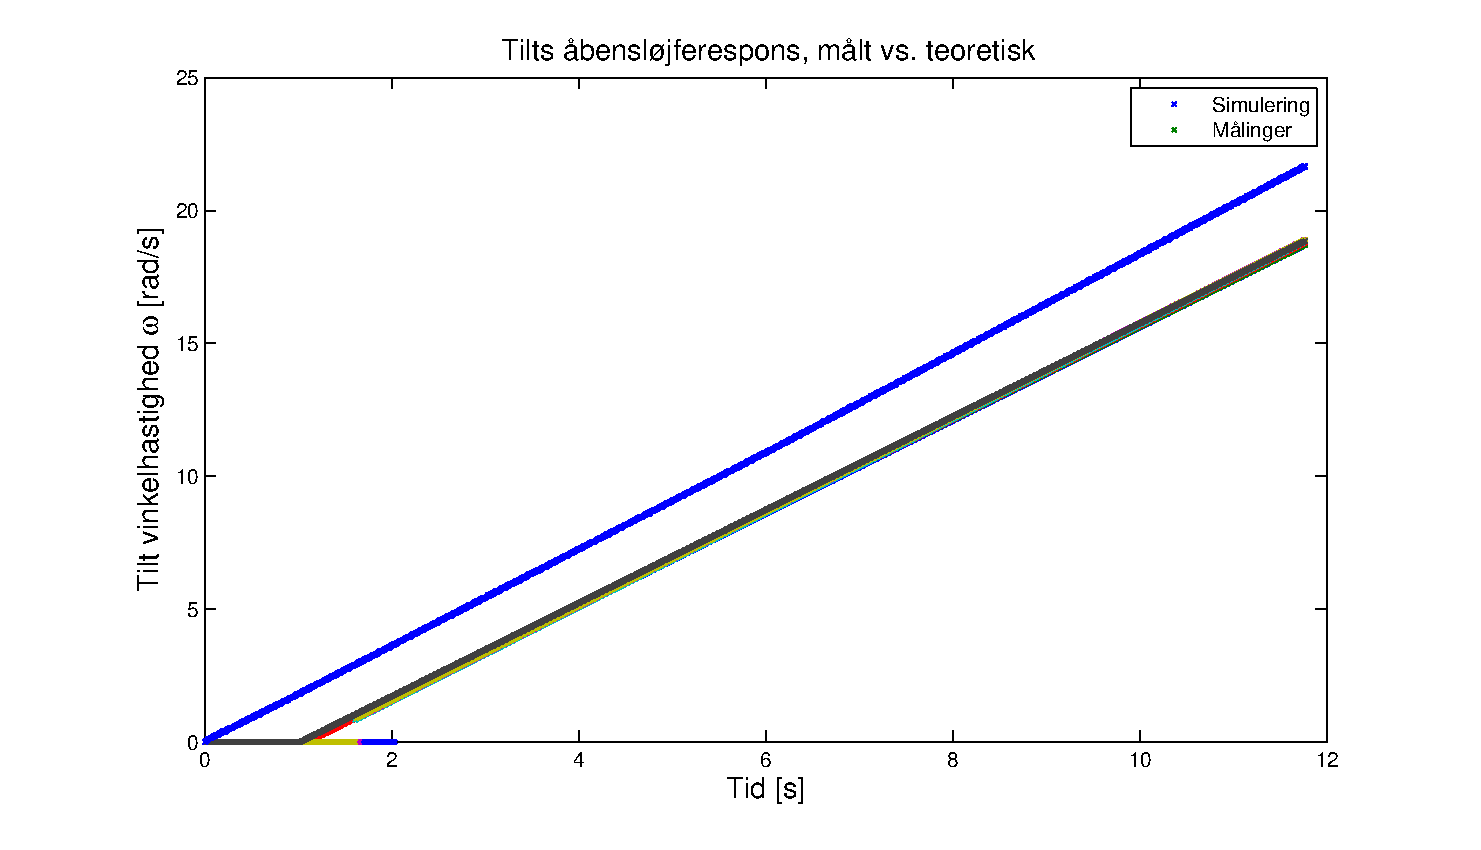
\includegraphics[width=1\textwidth]{./graphics/openloopVelocity1.eps}
	\caption[Tilt åbensløjferespons, målt vs. teoretisk]
		{Tilt åbensløjferespons, målt vs. teoretisk.
		Markeret med rødt er den målte respons for alle syv målinger,
		mens den teoretiske respons for de samme syv inputs er markeret med blåt.}
	\label{fig:openloopV1}
\end{figure}

Figur \ref{fig:openloopV1} viser den målte vinkelhastighed samt den teoretiske vinkelhastighed,
som forudsagt af overføringsfunktionen \(s\cdot{}G_{tilt}\).
Det ses på figur \ref{fig:openloopV1}, at den største afvigelse er en tidsforsinkelse.
Dette skyldes, at visse PWM-duty cycles ikke kan bevæge systemet.
Dødzonen af PWM-duty cycles, der ikke kan accelerere Tilt-systemet er målt til at befinde sig inden for
ca. \(\pm\) 12 \%, og for Pan-systemet til ca. \(\pm\) 10 \%.
Udover forsinkelsen fra dødzonen kan man på figur \ref{fig:openloopV1} aflæse
at den målte vinkelacceleration (hældningen af grafen) er marginalt mindre end den teoretiske.
Det antages, at denne opførsel hovedsageligt skyldes Coulomb-friktion.

Hvis man ønsker en mere nøjagtig matematisk model af Pan \& Tilt-systemet
er det altså en mulighed at indsætte dødzonen og evt. den ekstra dæmpning i modellen.
Det vælges dog at benytte åbensløjfeoverføringsfunktionerne \(G_{pan}\) og \(G_{tilt}\)
som udgangspunkt for analysen der hører til regulatordesignet,
og udvide modellen hvis regulatoren ikke lever op til kravene.

\subsection{Koordinattransformation}
\label{sec:koordinattransformation}
De kartesiske koordinater \(P_c=\left[x, y, z\right]\) skal transformeres til sfæriske koordinater \(P_s=\left[\rho \text{ ; } \phi \text{ ; } \theta\right]\), hvor \(\phi\) og \(\theta\) bruges som vinkelbestemmelserne for hhv. tilt og pan og \(\rho\) er afstanden fra PTS til duen som funktion af tiden.
Til trackingen er kun \(\phi\) og \(\theta\) nødvendige.
Positionbestemmelsen som funktion af tiden for det kartesiske koordinatsæt er udredt i afsnit \ref{subsubsec:para}.
Idet vinklerne skal bestemmes i forhold til PTS's rotationscenter og ikke koordinatsystemets origo, skal PTS's rotationscenter trækkes fra; \(PTS=[\text{19,2 ; 0 ; 0,45}]\). 

\subsubsection{Kartesiske koordinater}
Koordinattransformationen tager udgangspunkt i den kartesiske stedvektor \(Pos\left(t\right) \), ligning \ref{eq:pf:vektorparabel3d} samt PTS's offset, ligning \ref{eq:pf:stedvektorparabel}.
\begin{align}
\begin{split}
{ P }_{ c }=Pos\left( t \right) -PTS = \left( \begin{matrix} - 9,34\cdot t-13,7 \\32,851\cdot t-19,3
\\-{ 4,91\cdot t }^{ 2 }+5,473\cdot t+2,6\end{matrix} \right) [\text{m}]
\label{eq:pf:stedvektorparabel}
\end{split}
\end{align}
%Før koordinattransformationen fra kartesiske til sfæriske koordinater vises et grafisk overblik af \(\phi\) og \(\theta\) %samt \(\rho\), figur \ref{fig:thetaphi_degree}. 
Sammenhængen mellem de kartesiske og de sfæriske koordinater kan ses på fig \ref{fig:thetaphi_degree}. 
Grundet PTS's offset er origo for det sfæriske koordinatsystem PTS's rotationscenter (skæringspunktet mellem de to rotationsakser).

\begin{figure}[!th]
\centering
\begin{tikzpicture}[scale=4]
\include*{./graphics/3d_in_xyz_plane}
\end{tikzpicture}
\caption[Sfærisk koordinatsystem til koordinattransformation]{Viser duens placering i det sfæriske rum som funktion af  \(\phi\), \(\theta\) og \(\rho\).}
\label{fig:thetaphi_degree}
\end{figure}

\subsubsection{Sfæriske koordinater}
Som det fremgår af problemformuleringen modtager PTS lerduens
position som kartetiske koordinationer med en frekvens på 120 [Hz].
Dette bevirker at transformationen fra kartesiske koordinater til
sfæriske koordinater gøres ud fra nedenstående ligning \ref{eq:sv_koordi}.
\begin{align}
\begin{split}
{ P }_{ s } =\left( \begin{matrix} \rho  \\ \phi  \\ \theta  \end{matrix} \right) =\left( \begin{matrix} \sqrt { { { P }_{ c_{ x } } }^{ 2 }+{ { P }_{ c_{ y } } }^{ 2 }+{ { P }_{ c_{ z } } }^{ 2 } }  \\ { tan }^{ -1 }\left( \frac { \sqrt { { { P }_{ c_{ x } } }^{ 2 }+{ { P }_{ c_{ y } } }^{ 2 } }  }{ { P }_{ c_{ z } } }  \right)  \\ { tan }^{ -1 }\left( \frac { { P }_{ c_{ y } } }{ { P }_{ c_{ x } } }  \right)  \end{matrix} \right) %\\
 %&=\left( \begin{matrix} \sqrt { { \left( -9,34\cdot t-13,7 \right)  }^{ 2 }+{ \left( 32,851\cdot t-19,3 \right)  }^{ 2 }+{ \left( -{ 4,91\cdot t }^{ 2 }+5,473\cdot t+2,6 \right)  }^{ 2 } }  \\ { tan }^{ -1 }\left( \frac { \sqrt { { \left( -9,34\cdot t-13,7 \right)  }^{ 2 }+{ \left( 32,851\cdot t-19,3 \right)  }^{ 2 } }  }{  -{ 4,91\cdot t }^{ 2 }+5,473\cdot t+2,6 }  \right)  \\ { tan }^{ -1 }\left( \frac { 32,851\cdot t-19,3 }{ -9,34\cdot t-13,7 }  \right)  \end{matrix} \right) 
\label{eq:sv_koordi}
\end{split}
\end{align}
hvor \(\rho\) er afstanden i meter, \(\phi\) og \(\theta\) er angivet i grader, \citep[Kap. 10.6]{adam}.

\section{Koordinattransformation}
\label{sec:koordinattransformation}


\citep[Kap. 10.6, s. 598]{adam}
\section{Regulator}
\label{sec:kontrollerdeign}
Det er valgt at designe regulatoren efter processen illustreret i figur \ref{fig:designproces}.
\begin{figure}[!th]
\centering
\include*{./graphics/designproces}
\caption[Designprocessen]{Designprocessen, \citep{reg_modern_control_systems}.}
\label{fig:designproces}
\end{figure}
Formålet med reguleringen er som beskrevet i afsnit \ref{sec:problemformulering},
at kontrollere pan- og tilt-rammernes position, så de tracker en lerdue.
Dette gøres ved styring af deres hastighed, ved at justere spændingsfaldene over de
to DC-motorer. Spændingsfaldene styres af PWM-generatorer, og regulatoren
kan derfor styre motorernes hastighed ved at vælge PWM-signalernes duty cycles.

I afsnit \ref{sec:kravspecifikation} opstilles kravene til systemets respons.
Disse er for en 1-radian reference opsummeret nedenfor.
\begin{itemize}
\item \(t_{s} \leq 0,557 \mathrm{\left[s\right]}\) (Settling Time)
\item \(SSE \leq 1,78 \%\) (Steady State Tracking Error)
\item \(P.O. \leq 134 \%\) (Overshoot i procent)
\end{itemize}

Det er fastlagt i projektoplægget, at regulatoren skal implementeres på mikrocontrolleren.
Da systemet som input modtager kartesiske koordinater,
skal der også på mikrocontrolleren foregå en koordinattransformation
til den logiske vinkelrepræsentation med sfæriske koordinater.
Systemets konfiguration består altså af en koordinattransformation,
en regulering, en aktuering og en positionsmåling, som illustreret
i figur \ref{fig:digitalkontroller1}.
Bemærk at denne konfiguration er for ét SISO-undersystem (enten pan eller tilt),
og at mikrocontrolleren skal regulere begge SISO-undersystemer.
\begin{figure}[!th]
\centering
\begin{tikzpicture}[auto, node distance=2.6cm,>=latex']
\include*{./graphics/digitalkontroller1}
\end{tikzpicture}
\caption[Systemkonfiguration]{Systemkonfiguration}
\label{fig:digitalkontroller1}
\end{figure}
Som beskrevet i afsnit \ref{sec:problemformulering},
så er input-samplingen fastlagt til at foregå med en frekvens på 60 [Hz].
Men som illustreret på figur \ref{fig:digitalkontroller1}, så skal reguleringssløjfen
"køres" (sample) med en frekvens \(f_s=\frac{1}{T_s}\), der ikke nødvendigvis er 60 [Hz].
Dvs. A/D- og D/A-konverteringerne skal foregå med frekvensen \(f_s\).

Der er overordnet to strategier til valg af samplingfrekvensen \(f_s\) hvormed
reguleringssløjfen skal køre.
Hvis man designer en kontinuert regulator til det kontinuerte domæne, så
skal diskretiseringen af controlleren være så tæt på den kontinuerte regulator som muligt.
Det vil sige, samplingfrekvensen skal vælges så høj som mulig.
Hvis man derimod designer en diskret regulator til det diskrete domæne,
så er diskretiseringen allerede foretaget inden designet af regulatoren.
Dvs. man finder en diskretiseret model af det fysiske system inden designet af regulatoren.
Kravet til diskretiseringen af åbensløjfeoverføringsfunktionerne er, at den diskrete repræsentation
skal være tilfredsstillende tæt på de kontinuerte overføringsfunktioner.
Hvis den diskrete overføringsfunktion eksempelvis afviger 20 \% fra den kontinuerte, ville man
sandsynligvis overveje at benytte en højere samplingfrekvens til diskretiseringen.
Sammenligningen af den diskrete overførselsfunktion og den kontinuerte overføringsfunktion
kan være både i tidsdomænet (fx steprespons) og i frekvensdomænet (frekvensrespons, fx. Bode-plots).




\begin{figure}[!th]
\centering
\begin{tikzpicture}[auto, node distance=2.6cm,>=latex']
\include*{./graphics/digitalkontroller2}
\end{tikzpicture}
\caption[tekst i indholdsfortegnelsen]{figurtekst}
\label{fig:}
\end{figure}

\begin{figure}[!th]
\centering
\begin{tikzpicture}[auto, node distance=2.6cm,>=latex']
\include*{./graphics/digitalkontroller3}
\end{tikzpicture}
\caption[tekst i indholdsfortegnelsen]{figurtekst}
\label{fig:}
\end{figure}
\part{Implementering}
\todo[inline, color = pink, author = Mikkel]{Her bør også være en introduktion til hvad der skrives om i afsnittet og hvorfor. Kunne måske hjælpe til følelsen af en rød tråd igennem rapporten.}

\section{Mikrocontroller}
\label{sec:mikrocontroller}
%
\subsection{Krav til mikrocontrolleren}
\todo[inline, author=Michael]{Husk at TEST sektionen skal se om vi opfylder disse krav. Hvis ikke vi tester tingene skal de slettes fra dette afsnit!!!}
Mikrocontrolleren har følgende opgaver: 
%\todo[inline, author=Michael]{YOU CANT TOUCH THIS - lad mig lige skrive færdig!}
%\todo[inline, author=Michael]{Denne sektion mangler generelt at blive forkortet. }
%\todo[inline, author=Michael]{Anders, kan vi ændre layouttet så listerne ikke tager så meget plads? }


\begin{itemize}
\itemsep1pt
	\item Afvikling af regulatorerne.
	\item Kommunikation med FPGA vha. SPI.
	\item Modtage kommandoer fra PC'en via UART.
	\item Sende relevant data til brugeren via UART.
\end{itemize}

Regulatorerne skal afvikles i hård realtid\footnote{Dvs. at tasken skal afvikles, inden dens deadline - inden for en periode.}, da det ellers er vanskelligt at modellere forsinkelsen matematisk.


SPI\footnote{Serial Peripheral Interface, også kaldet SSI} bruges til at overføre PTS's position fra FPGA til mikrocontroller. Desuden overføres beregnet duty-cycle fra mikrocontroller til FPGA. Kommunikationen skal være tilpas hurtig, så regulatorerne ikke beregner på forældet data. Forsinkelsen for overførsel af data fra begge motorer må ikke overstige 5\% af sampletiden. Ved $T_s = \frac{1}{600}$ er det: 
\begin{equation}
	T_{spi delay} = \frac{1}{600} \cdot 0.05 = 8,33 \cdot 10^{-5}[s]
\end{equation}


Systemet skal kunne modtage brugerinput gennem et terminalprogram. Brugerinterfacet er ikke tidskritisk. Der skal være mulighed for at udlæse væsentlige systemparametre. F.eks. PTS' position, ønsket position, aktuel Pwm duty cycle osv.

\todo[inline, author=Michael]{Måske skal disse systemparametre defineres mere fast.}

%\begin{itemize}
%\itemsep1pt
%	\item PTS' position. 
%	\item Ønsket position. 
%	\item Afvigelse fra ønsket position. 
%\end{itemize}

Desuden skal systemet gemme disse informationer i en log-fil, som kan udlæses efter systemet er færdig med at tracke målet. 

Systemet skal kunne reagere på følgende bruger inputs:


\begin{itemize}
\itemsep1pt
	\item Start tracking
	\item Stop tracking
	\item Reset systemet
	\item Gå til koordinat (x,y,z)
	\item Set PWM
	\item Læs log
\end{itemize}

%%%%%%%%%%%%%%%%%%%%%%%%%%%%%%%%%%%%%%%%%%%%%%%%%%%%%

\subsection{Beskrivelse af valgt(?) mikrocontroller.}
Den udleverede mikrocontroller er en 32 bit Stellaris LM3S6965, baseret på en ARM Cortex M3 kerne. Den opererer ved 50 [MHz] og bruger Thump 2 instruktionssættet. Den indeholder 256 [kB] flash hukommelse samt 64 [kB] SRAM. 
\citep{lm3s6965}

SPI er indbygget som et hardwaremodul, med seperate FIFO buffere til afsendelse og modtagelse. Hardwaren sender data fra den ene den buffer og lægger modtaget data i den anden. Derfor er det ikke nødvendigt for programmøren at holde styr på timingen. Størrelsen af hvert dataframe kan være 4 - 16 bits. 

UART er også implementeret som et hardwaremodul. Modulet indeholder seperate FIFO buffere til afsendelse og modtagelse af data, hver med plads til 16 datawords (max 8 bit). 
\todo[inline, color = pink, author = Mikkel]{Max 8 bit?}


%%%%%%% Den næste sætning er vist bare fyldtekst
%Controlleren indeholder også et væld af hardwaremoduler til andre funktioner, men disse er ikke relevante for projektet.

%%%%%%%%%%%%%%%%%%%%%%%%%%%%%%%%%%%%%%%%%%%%%%%%%%%%%

\subsection{Valg af skedulering/operativsystem}
Der er undersøgt 4 forskellige muligheder for skedulering: 

\begin{itemize}
\itemsep1pt
	\item CoOS\footnote{\citep{www.coocox.com/CoOS.htm}} 
	\item freeRTOS\footnote{\citep{freertos.org}}
	\item Run-To-Complete-Scheduler\footnote{Introduceret i EMP-kurset}
	\item Super-loop
\end{itemize}

De to førstnævnte er fulde operativsystemer med flere mulige skeduleringsalgoritmer. 
Til valget er der lagt vægt på følgende parametre: 

\begin{itemize}
\itemsep1pt
	\item Opfylder kravene til realtidsafvikling af regulatorerne. 
	\item Muligheden for at (gen)bruge elementer fra EMP-kurset.
\end{itemize}

\begin{table}[h!]
\begin{tabular}{|l|l|l|l|l|}
\hline 
 & coOS & freeRTOS & RTCS & Super loop \\ 
\hline 
Skedulering & Preemptive priority  & Preemptive priority  & Non-preemptive & Non-preemptive  \\ 
			& /round robin		&	/round robin & &	\\
\hline 
Queues & Ja & Ja & Nej & Nej \\ 
\hline 
Semaphore & Counting og Binære  & Counting og Binære & Binære  & Nej  \\ 
\hline 
Introduceret & Nej & Ja & Ja & Ja \\ 
i EMP kurset &   &   &   &   \\
\hline 
\end{tabular} 
\caption{Specifikationer for de undersøgte systemer}
\label{tb:os_comparison}
\end{table}
\todo[inline, author=Michael]{Ikke færdig - tilføj noget om hvor lang tid et context switch tager. Dispatch latency.}
%
\subsection{Implementering}
%disp: 
% task diagram
% beskrivelse af tasks
% implementering af enkelt task (CONTROL TASK). 
%   - hvordan sikres at denne kører realtid.
% 
% beskrivelse af interfacet
% 
\todo[inline, author=Michael]{Venter på at kodens struktur er helt færdig - inden da giver det ikke mening at skrive dette afsnit færdigt. }

Valget af freeRTOS som operativsystem gjorde det muligt at opdele programmet i seperate tasks. Taskdiagrammet er vist på figur \ref{fig:task_diagram}. 

% TASK DIAGRAM
\begin{figure}[!h]
\centering
\begin{tikzpicture}[node distance = 3.2cm]
	\include*{./graphics/uc_task_diagram}
\end{tikzpicture}
\caption[Task diagram]{Taskdiagrammet viser programmets opdeling i tasks.}
\label{fig:task_diagram}
\end{figure}

\subsubsection{Beskrivelse af de enkelte tasks}
\begin{description}
\itemsep-3pt
	\item[UART] Grundet UART hw. bufferen kun indeholder 16 pladser \citep[Side. 430]{lm3s6965}. Sørger en Send og Recieve task for at sende data videre. Ekstra Semaphore til at sikre kun en task kan skrive til Uart af gangen er implementeret.
	\item[Interface] Tolker på brugerinputs og sender relevante kommandoer til Control tasken.
	\item[Control] Afvikler regulatorerne. Se mere indgående beskrivelse i sektion \ref{sec:control_task}. Denne task afvikles i realtid, med en frekvens på 600 Hz. 
	Denne task sørger for at SPI Kommunikationen med FPGA'en bliver afviklet på de rigtige tidspunkter.
	\item[Logger] Denne task opdaterer logfilen med data fra "status" køen.
\end{description}

\subsubsection{Interface task}
\label{sec:interface}
Bruger Interfacet gør det overskueligt at styre og skifte mellem de forskellige tilstande som systemet kan køres i.
Der er lavet funktioner som bruges til test af specifikke funktioner og funktioner som starter en større test.
Formålet er at gøre det simpelt for gruppen, det er altså ikke tænkt til en kunde som ikke ved noget om systemet.
Fjernelse af implementerede funktioner for at gøre det simpelt har ikke været en prioritet. 
De primære funktioner er at sætte en position eller starte tracking af lerduen.
Hvis det indtastede ikke bliver genkendt bliver en liste over gyldige funktioner udskrevet.

\begin{table}[h!]
\begin{tabular}{|l|l|l|}
\hline 
Kommando: & Funktion: & Parametre: \\ 
\hline 
read & Slå log til eller fra.  &   \\ 
\hline 
start & Start tracking af lerdue &   \\ 
\hline 
stop & Stop systemet &   \\ 
\hline 
open & Start åben sløjfe test &   \\ 
\hline 
reset & Gå til udgangsposition &   \\ 
\hline 
C xxx.yyy.zzz & Gå til  kartesisk koord. (x,y,z) & x,y,z = Koordinaterne i meter \\ 
\hline 
A aaaa.bbbb & Gå til sfærisk koord.  & a = Tilt, b = Pan, begge i ticks. \\ 
\hline 
Pmfxx & Sæt dutycycle for motor m & m = Motor ("A" ell. "B"), \\ 
  & & f = fortegn ($+$ ell. $-$),  \\
  & & xx = PWM dutycycle i \%\\
\hline 
\end{tabular} 
\caption{Viser UART-interfacets kommandoer.}
\label{tb:uart_interface}
\end{table}



\subsubsection{Control task}
\label{sec:control_task}

Control tasken henter et koordinat, transformerer koordinatet udregner en PWM med PID controlleren og opdaterer loggen.
hver gang control tasken bliver kørt bliver der hentet en position ind over SPI og sendt ny PWM. 
Control tasken ved hvilke ting som er relevant at gemme i loggen, så ved start af tracking bliver positioner og pwm gemt i loggen.
I kodeudsnittet \ref{ctrl_task} ses der tasken som den bliver kørt hvis den er i tracking stadiet.

\lstinputlisting[language=c, 
        firstnumber=120,
        firstline=120, 
        lastline=122,
        ]{codeexample/ctrl_task.c}
\(\vdots\)
\lstinputlisting[language=c, 
        firstnumber=155,
        firstline=155, 
        lastline=163,
        ]{codeexample/ctrl_task.c}
\(\vdots\)
\lstinputlisting[language=c, 
        firstnumber=180,
        firstline=180, 
        lastline=186,
        caption={ af ctrl\_task.c.\label{ctrl_task}}
        ]{codeexample/ctrl_task.c}
        
\subsubsection{SPI}
\label{sec:spi-implementering}
Det blev vedtaget at mikrocontrolleren var masteren og FPGA'en blev slaven, da FPGA'en helst skulle være så enkel som mulig.

Mikrocontrolleren har indbygget tre forskellige versioner af SPI. De tre typer er TI Synchronous Serial Frame Format (SSFT), Freescale og Microwire. 
%Til at overfører data mellem Mikrocontrolleren og FPGA’en skal der bruges en enkel protokol med full duplex. \todo[author=Anders]{Hovedgrundene til valget af SPI protokol.}
%Hovedgrundene for at protokollen skal være enkel, er at der ikke sendes meget data, dataene er enkel, og afstanden, den sendes, er kort. 
%Microwire er ikke full duplex. Så det er enten SSFt eller Freescale, der skulle bruges. Da SSFT havde færre opsætningsmuligheder, blev den valgt som protokol. 
%I SSFT ligger svaret på nogle af overvejelserne. Overvejelserne har været om MOSI skal trigger på rising eller falling edge, og hvordan Slave Select skulle opføre sig.
Microwire blev udelukket da den ikke er full-duplex og dermed ikke en ren SPI standard. 
Freescale formatet blev udelukket da opsætningen af denne var mere kompliceret end for SSFT, uden at tilføje ekstra muligheder.

\todo[author=Åse,inline]{kan omfomulere Microwire blev...}

\begin{figure}[th!]
\centering
\begin{tabular}{c|c|c|c|c}
1 motorbit &1 retningsbit & 1 set PWMbit & 2 ignored bits & 11 PWM dutycyclebits\\
\end{tabular}
 \begin{tabular}{c|c|c}
 1 motorbit & 4 ignored bits & 11 decoderbits
 \end{tabular}
\captionsetup{type=figure}
\caption[SPI framestruktur]{Øverst ses framestrukturen fra mikrocontrolleren til FPGA'en. Nederst ses framestrukturen fra FPGA'en til mikrocontrolleren.}
\label{tb:protokol1}
\end{figure}

\todo[author=Åse,inline]{Skriv en figur tekst senere} 

\todo[inline, author=Michael]{Alternativ version. Please vote :)}
\todo[inline, author=Nikolaj]{Jeg stemmer på nummer 2:)}

\begin{figure}[h!]
\centering
\subfloat[Mikrocontroller til FPGA.\label{fig:spi_to_fpga}]{%
\begin{tabular}{|c|}
    \hline
    Motor (1 bit) \\
    \hline
    Retning (1 bit) \\
    \hline
    Set PWM (1 bit) \\
    \hline
    N/A (2 bit) \\
     \\
    \hline
     \\ \\ \\ \\
    PWM duty cycle \\
    (11 bits) \\ \\ \\ \\ \\
    \hline
  \end{tabular}
}
\qquad
\subfloat[FPGA til Mikrocontroller.\label{fig:spi_from_fpga}]{%
\begin{tabular}{|c|}
    \hline
    Motor (1 bit) \\
    \hline \\
    N/A (4 bit) \\
     \\ \\
    \hline
     \\ \\ \\ \\
    PWM duty cycle \\
    (11 bits) \\ \\ \\ \\ \\
    \hline
  \end{tabular}
}
\caption[Lerduens parabel i 2D]{Viser parablen af lerduens bane i 2D.}
\end{figure}


Størrelse af data framen blev valgt til 16 bit ($2^4$), da det giver mulighed for at sende motorens hastighed og deres position (begge 11 bit) samt kontroldata. Opbygningen af de to datawords kan ses på figur\ref{tb:protokol1}.
På Figur "microC til FPGA" kan man se dataword'et der bliver sendt fra Mikrocontrolleren. Mikrocontrolleren sender den  PWM, der skal sættes på den bestemte motor i den bestemte retning. Det er det motor- og retningsbittene bestemmer.
Da SPI er full duplex skal der sendes data fra både Mikrocontrolleren og FPGA’en, FPGA’en kan ikke sende data uden at Mikrocontrolleren også gør det. På Mikrocontrolleren ville man gerne kunne få en position uden, at den sætter en ny PWM. Derfor skal der bruges en bit, hvor FGPA’en kan se om den skal sætte PWM’en, eller om den kun skal sende information tilbage. Der er det PWMset bruges til.
På figur "microC til FPGA" ses dataword'et som FPGA'en sender. FPGA'en sender positionen på den bestemte motor.


\subsection{Test} 
% Test af SPI overførsel
% Test af realtidsafvikling af reguleringssløjferne, 
% lever vi op til kravene?
% 





\subsection{Delkonklusion}

\section{FPGA}
\label{sec:FPGA}

\todo[inline]{Mikkel: Er slet ikke færdigt, så lad venligst være med at rette eller andet.}
FPGA'en er leddet mellem microcontrolleren og motorene på PTS. 
Kommunikationen mellem FPGA og microcontroller skal ske ved hjælp af SPI. 
FPGA'en skal producere PWM signal til motorerne på PTS og skal kunne tælle motorenes rotationer. 
FPGA'en er i projeket et BASYS board \footnote{DIGILENT BASYS 2}, der programmeres ved brug af VHDL.

\subsection{Struktur}
Det er forsøgt at bygge funktionaliteter op ved at skrive generiske komponenter. 

\subsection{PWM}
Der skal fra FPGA'en genereres PWM signaler til at styre motorerne på PTS.
\subsubsection*{Valg af PWM frekvens}
Det ønskedes at have en PWM frekvens, der ikke ligger i det hørbare område. 
Det ønskedes også at have en god opløsning på PWM. 
Ved 11 bit og brug af BASYS boardets interne clock på 50 MHz bliver PWM frekvensen passende høj:
\begin{equation}
  \frac{2^{11}}{50 MHz} = 24.41 KHz 
\end{equation}

\begin{figure}[!th]
\centering
\begin{tikzpicture}[node distance = 5 cm,scale=1]
\include*{./graphics/FPGA_blok}
\end{tikzpicture}
\caption[tekst i indholdsfortegnelsen]{figurtekst.}
\label{fig:FPGA_blok}
\end{figure}
\todo[author=Anders,inline]{Jeg skal lige have tjekket op med nikolaj omkring forbindelsen til Decoder til output decoder.}

\section{Kommunikation mellem mikrocontroller og FPGA}

\subsection{Overvejelser og valg}
%%%%% FYLDTEKST:
%Der er gået mange overvejelser i hvordan SPI'en mellem mikrocontrolleren og FPGA'en skal opbygges.

Det blev vedtaget at mikrocontrolleren var masteren og FPGA'en blev slaven, da FPGA'en helst skulle være så enkel som mulig.

Mikrocontrolleren har indbygget tre forskellige versioner af SPI. De tre typer er TI Synchronous Serial Frame Format (SSFT), Freescale og Microwire. 
%Til at overfører data mellem Mikrocontrolleren og FPGA’en skal der bruges en enkel protokol med full duplex. \todo[author=Anders]{Hovedgrundene til valget af SPI protokol.}
%Hovedgrundene for at protokollen skal være enkel, er at der ikke sendes meget data, dataene er enkel, og afstanden, den sendes, er kort. 
%Microwire er ikke full duplex. Så det er enten SSFt eller Freescale, der skulle bruges. Da SSFT havde færre opsætningsmuligheder, blev den valgt som protokol. 
%I SSFT ligger svaret på nogle af overvejelserne. Overvejelserne har været om MOSI skal trigger på rising eller falling edge, og hvordan Slave Select skulle opføre sig.
Microwire blev udelukket da den ikke er full-duplex og dermed ikke en ren SPI standard. 
Freescale formatet blev udelukket da opsætningen af denne var mere kompliceret end for SSFT, uden at tilføje ekstra muligheder. 

Frekvensen af SCLK skal vælges så høj, at SPI ikke bliver en flaskehals i kommunikationen mellem mikrocontrolleren og FPGA’en, og tilpas lav, så der ikke introduceres unødige fejlkilder, ved at FPGA’en ikke kan følge med.
\todo[inline, author=Michael]{Linjen herover bør fjernes da det er bedre at kravene ud fra vores krav til control-tasken som helhed. Se uC afsnittet under kravspecifikation.}

\todo[author=Åse,inline]{Hvad er SCLK's frekvens}
\todo[author=Anders,inline]{Eventuelt skal nedenstående ind i næste afsnit.}
Størrelsen af framen skulle være så stor, at PWM kan sendes til FPGA’en, og positionen i form af ticks kan sendes fra FPGA’en. Begge skal kunne sendes i den rigtige opløsning. PWM og ticks har begge en størrelse af 11 bit. Der skal også være et motor, retnings- og PWMset bit. Det giver at framen mindst skal være 14 bit lang. Mikrocontrolleren understøtter en størrelse mellem fire og 16 bit.16 bit blev valgt, da der er plads til udbygning.
\todo[inline, author=Michael]{Forkort dette afsnit. F.eks:}
Størrelse af data framen blev valgt til 16 bit ($2^4$), da det giver mulighed for at sende motorens hastighed og deres position (begge 11 bit) samt kontroldata. Indholdet af de enkelte pakker/datawords kan ses på figur \label{tb:protokol1}.

\subsection{Brugen af SPI}



\todo[author=Åse, inline]{Det tekniske om Mikrocontroller er meget kort. Men det er noget der bare kan læses i databladet. Skal der henvises til databladet.}

På mikrocontrolleren bruges SPI verion SSFT. Den er sat til at være master, derfor er det den, som initialiserer overførelsen mellem mikrocontrolleren og FPGA'en, \citep[Kap. 13]{lm3s6965}.

På FPGA'en er SPI'en tp shift registre, der konverterer signalet fra seriel til parallel og vice versa. Efter konverteringen sendes det videre ind i systemmet. 

\begin{figure}[!th]
\centering
\begin{tikzpicture}[scale=1]
\include*{./graphics/SPIfigur}
\end{tikzpicture}
\caption[tekst i indholdsfortegnelsen]{figurtekst}
\label{fig:signal_SPI}
\end{figure}

Det er en enkel protokol som bliver brugt uden tjeksum eller nogen anden form for administration. Frame størrelse er på 16 bit. På figur \ref{fig:signal_SPI} kan man se opbygningen af både framen der bliver sendt til FPGA’en og til Mikrocontrolleren. Til FPGA’en bliver der sendt den PWM, der skal sættes på den bestemte motor i den bestemte retning. Det er det motor- og retningsbittene bestemmer. Da SPI er full duplex skal der sendes data fra både Mikrocontrolleren og FPGA’en, FPGA’en kan ikke sende data uden at Mikrocontrolleren også gør det. På Mikrocontrolleren ville man gerne kunne få en position uden, at den sætter en ny PWM. Derfor skal der bruges en bit, hvor FGPA’en kan se om den skal sætte PWM’en, eller om den kun skal sende information tilbage. Der er det PWMset bruges til. Hvis den er høj bliver framen kasseret, men hvis den er lav bliver PWM’en sat. Framen der bliver sendt til mikrocontrolleren er positionen på den bestemte motor. Framen ses i nedenstående figur \ref{tb:protokol1}. Øverst ses framestrukturen fra mikrocontrolleren til FPGA'en og nederst ses framestrukturen fra FPGA'en til mikrocontrolleren. 

\begin{figure}[th!]
\centering
\begin{tabular}{c|c|c|c|c}
1 motorbit &1 retningsbit & 1 set PWMbit & 2 ignored bits & 11 PWM dutycyclebits\\
\end{tabular}
 \begin{tabular}{c|c|c}
 1 motorbit & 4 ignored bits & 11 decoderbits
 \end{tabular}
\captionsetup{type=figure}
\caption[SPI framestruktur]{Øverst ses framestrukturen fra mikrocontrolleren til FPGA'en. Nederst ses framestrukturen fra FPGA'en til mikrocontrolleren.}
\label{tb:protokol1}
\end{figure}

   
  
 % Fra FPGA til Mikrokontroller format:
 %\begin{figure}[th!]
 %\centering
 %\begin{tabular}{c|c|c}
 %1 motorbit & 4 ignored bits & 11 decoderbits
 %\end{tabular}
 %\captionsetup{type=figure}
 %\caption[tekst i indholdsfortegnelsen]{tabeltekst}
 %\label{tb:protokol2}
 %\end{figure}

%\part{Regulator justering og PTS verifikation}
\part{Regulator justering}
I denne del optimeres performance ved at ændre på regulatorene for pan og tilt.
Herefter vurderes PTS's performance i forhold til kravspecifikationen.
\section{Justering ift. matematisk model af PTS}
\label{ss:regulatorMat}
Som beskrevet i afsnit \ref{ss:ValgReg} er det valgt at implementere to PI-regulatorer.
Der tages udgangspunkt i den matematiske model af systemet, bestående af overføringsfunktionerne
\(G_{tilt,zoh}\) og \(G_{pan,zoh}\), som er diskretiseringer af de kontinuerte overføringsfunktioner.
Der skal findes to sæt koefficienter, \(K_P\) og \(K_I\), et sæt til hver regulator.
For at medtage den væsentligste ulinearitet, dødzonen, i regulatordesignet,
er det valgt at simulere systemet i Simulink.
I Simulink er den diskretiserede overføringsfunktion indsat sammen med en model for dødzonen,
målt eksperimentelt, samt PI-regulatoren. Det simulerede systems blokdiagram er illustreret i figur \ref{fig:simulink1}.
Da modellen indeholder ulineariteter er det valgt at starte med et simpelt gain \(K_P\) på 1,
og med Trial-and-Error metoden prøve sig frem til koefficienterne.
Begge regulatorer gives et parabelinput, og deres performance vurderes
efter deres evne til at følge parablen. Dvs. det er forsøgt at minimere Tracking fejlen.


\begin{figure}[!th]
\centering
\begin{tikzpicture}[auto, node distance=2.6cm,>=latex']
%\begin{tikzpicture}[scale=0.9, every node/.style={scale=0.9}, node distance=2.6cm, =>latex']
\include*{./graphics/simulink1}
\end{tikzpicture}
\caption[Simuleret system]
		{Simuleret system. Tilbagekoblingsblokken angiver, at outputsignalet kvantiseres med et interval på \(q\mathrm{:} \frac{1}{1080}\),
		for at simulere motorens encoder feedback.
		\(D\left(z\right)\) er PI-regulatoren.}
\label{fig:simulink1}
\end{figure}


Med ovenstående metode blev koefficienterne i tabel \ref{tb:pidSimulink} fundet tilfredsstillende.
Koefficienterne i tabel \ref{tb:pidSimulink} benævnes startkoefficienterne, da regulatorjusteringen
ift. det fysiske system starter med disse værdier.
Tracking fejlen er afbildet i figur \ref{fig:pidSim1}, og som det ses af grafen, når den maks. 0,5 \degree{} i simuleringen.

\begin{figure}[h!]
\centering
\begin{tabu}{l|[1.25pt]c|c|c}
      & \(K_P\) & \(K_I\) & \(K_D\)\\\tabucline[1.25pt]{-}
Tilt  & 240 & 85 & -\\\hline%0,248960\\\hline
Pan   & 240 &  100 & -
\end{tabu}
\captionsetup{type=table}
\caption[Regulatorkoefficienter]{Koefficienter fundet vha. simulering.}
\label{tb:pidSimulink} 
\end{figure}

\begin{figure}[h!]
\centering
\includegraphics[width=1\textwidth]{./graphics/pidSim1.eps}
\caption[Tracking fejl ved simulering]{Tracking fejl ved simulering af PTS med regulatorkoefficienterne fra tabel \ref{tb:pidSimulink}.} 
\label{fig:pidSim1}
\end{figure}

De to regulatorer er med startkoefficienterne blevet afprøvet i praksis.
Figurer \ref{fig:pidPhys1} viser Pan-fejlsignalet (rød) og Tilt-fejlsignalet (blå)
i forhold til den kontinuerte lerdueparabel fra applikationen.

\begin{figure}[h!]
\centering
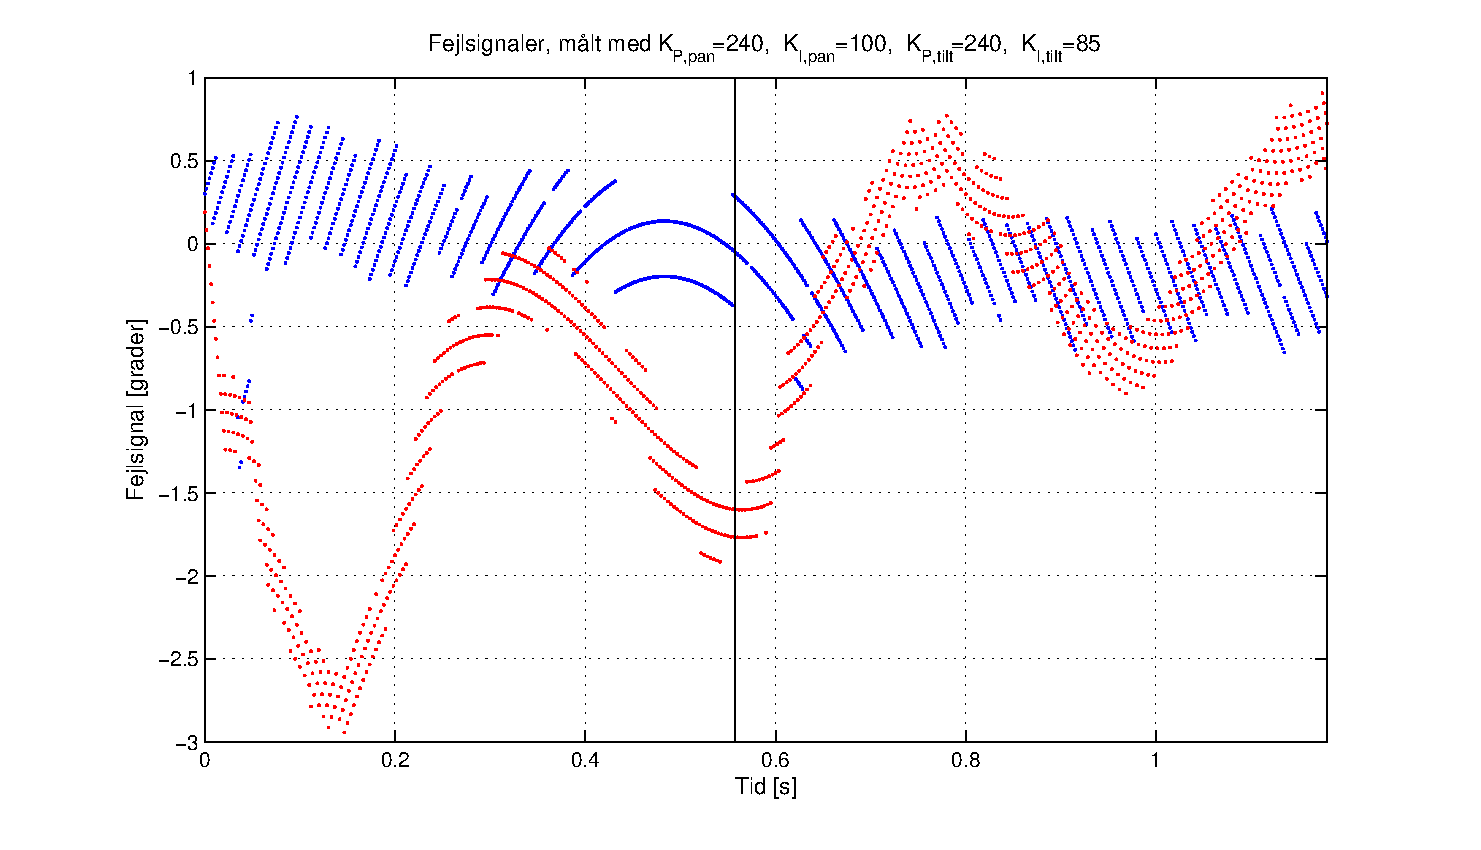
\includegraphics[width=1\textwidth]{./graphics/pidPhys1.eps}
\caption[Fejlsignaler m. startkoefficienter]{Fejlsignaler m. startkoefficienterne fra tabel \ref{tb:pidSimulink}.
	De sorte lodrette streger angiver \(t_s=0,557 \text{ [s]}\).\\
	Pan-fejlsignalet er markeret med prikker, og Tilt-fejlsignalet er markeret med krydser.} 
\label{fig:pidPhys1}
\end{figure}

Som det ses på figur \ref{fig:pidPhys1} giver regulatoren til Tilt et fejlsignal,
der maks. afviger 0,9 \degree{} fra 0.
Pan-fejlen afviger derimod op til 1,8 \degree{}.
Tracking fejlen er altså langt større end kravet på maksimalt 1,02 \degree.
En manuel justering af koefficienterne på især Pan-regulatoren er derfor nødvendig.

\section{Manuel justering ift. fysisk PTS}
Ved at ændre på koefficienterne og analysere fejlgraferne justeres performance 
hen mod det ønskede.

Det vurderes på baggrund af det lave fejlsignal ved Tilt at den i afsnit \ref{ss:regulatorMat} fundne
PI-regulator for Tilt er anvendelig i praksis.

På Pan er der behov for en hurtigere og mere dæmpet reaktion,
og det vurderes derfor, at der på Pan er brug for en PID-regulator.

\subsection{Valg af integratormætning}
Det vælges at sætte integratormætningen til 100 for begge regulatorer, da det vurderes, at der drages
fuld nytte af integratorleddet når ligning \ref{eq:integratorsaturation} 
overholdes.

\begin{equation}
	K_I \cdot Integrator_{Max} > PWM_{Max}
\label{eq:integratorsaturation} 
\end{equation}

\todo[inline,color=Pink,author=Mikkel]{Måske for kvalitativt. Måske må man ikke bare lave sin egen ligning, men jeg har ikke nogne kilde.}

\subsection{Tilføjelse af et D-filter}
Undervejs i den manuelle justering af PID-regulatoren til Pan blev det fundet, at D-leddet ikke udnyttedes til fulde,
og at kravene ikke kunne overholdes med PID-regulatoren som den var.
Det valgtes derfor at tilføje et filter til D-leddet. 
Det betyder at D-leddet nu vægter tidligere ændringer i fejlsignalet. 
Filtret reducerer peaks i det differrentierede fejlsignal, der skyldes Zero Order Hold i upsamplingen (se afsnit \ref{subsec:upsampling}).

Der implementeres et 4. ordens FIR filter. Filtret er designet i MATLAB's grafiske fdatool og gør brug af at Kaiser vindue.
Filtrets step- og frekvensrespons kan ses på figur \ref{fig:d_filter_step} hhv. \ref{fig:d_filter_bode}. 

\begin{figure}[h!]
\centering
\subfloat[Steprespons for det implementerede filter.\label{fig:d_filter_step}]{%
	\hspace*{-0.6cm}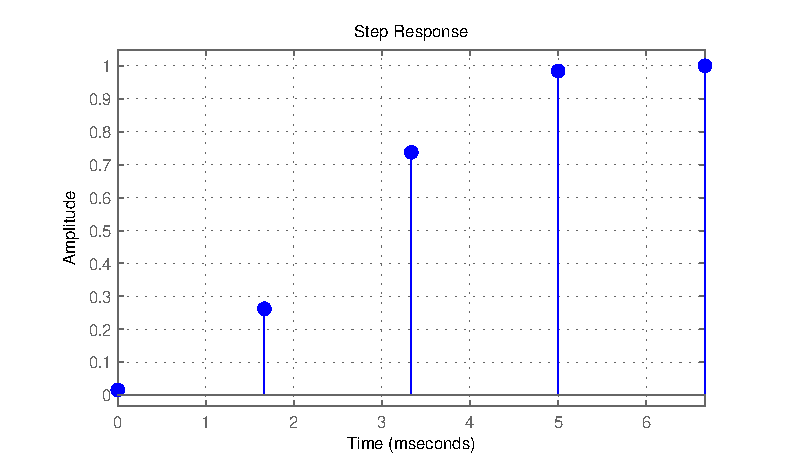
\includegraphics[width=0.57\textwidth]{./graphics/d-filter-step-small}
}
\subfloat[Frekvensrespons for det implementerede filter.\label{fig:d_filter_bode}]{%
	\hspace*{-1.15cm}\includegraphics[width=0.57\textwidth]{./graphics/d-filter-bode-small}
	
}
\caption[D-filterets respons]{Dette er ikke en figur tekst. }
\label{fig:d_filter}
\end{figure}

\section{Endelig performance}
Efter adskillige test og finjustering af regulatoren, vurderes det at 
koefficienterne i tabel \ref{tb:PID_final} giver den bedst mulige performance 
for PTS. Denne performance ses i \ref{fig:PID_final}. Det ses at trackingfejlen 
holder sig inden for de 1,02$\degree$  pånær ved et par enkelte samples.

\begin{figure}[h!]
\centering
\begin{tabu}{l|[1.25pt]c|c|c}
      & \(K_P\) & \(K_I\) & \(K_D\)\\\tabucline[1.25pt]{-}
Tilt  & 49 & 32,5 & 0\\\hline
Pan   & 80 & 160 & 3,55
\end{tabu}
\captionsetup{type=table}
\caption[Endelige regulatorkoefficienter]{De endelige regulatorkoefficienter.}
\label{tb:PID_final} 
\end{figure}

\begin{figure}[h!]
\centering
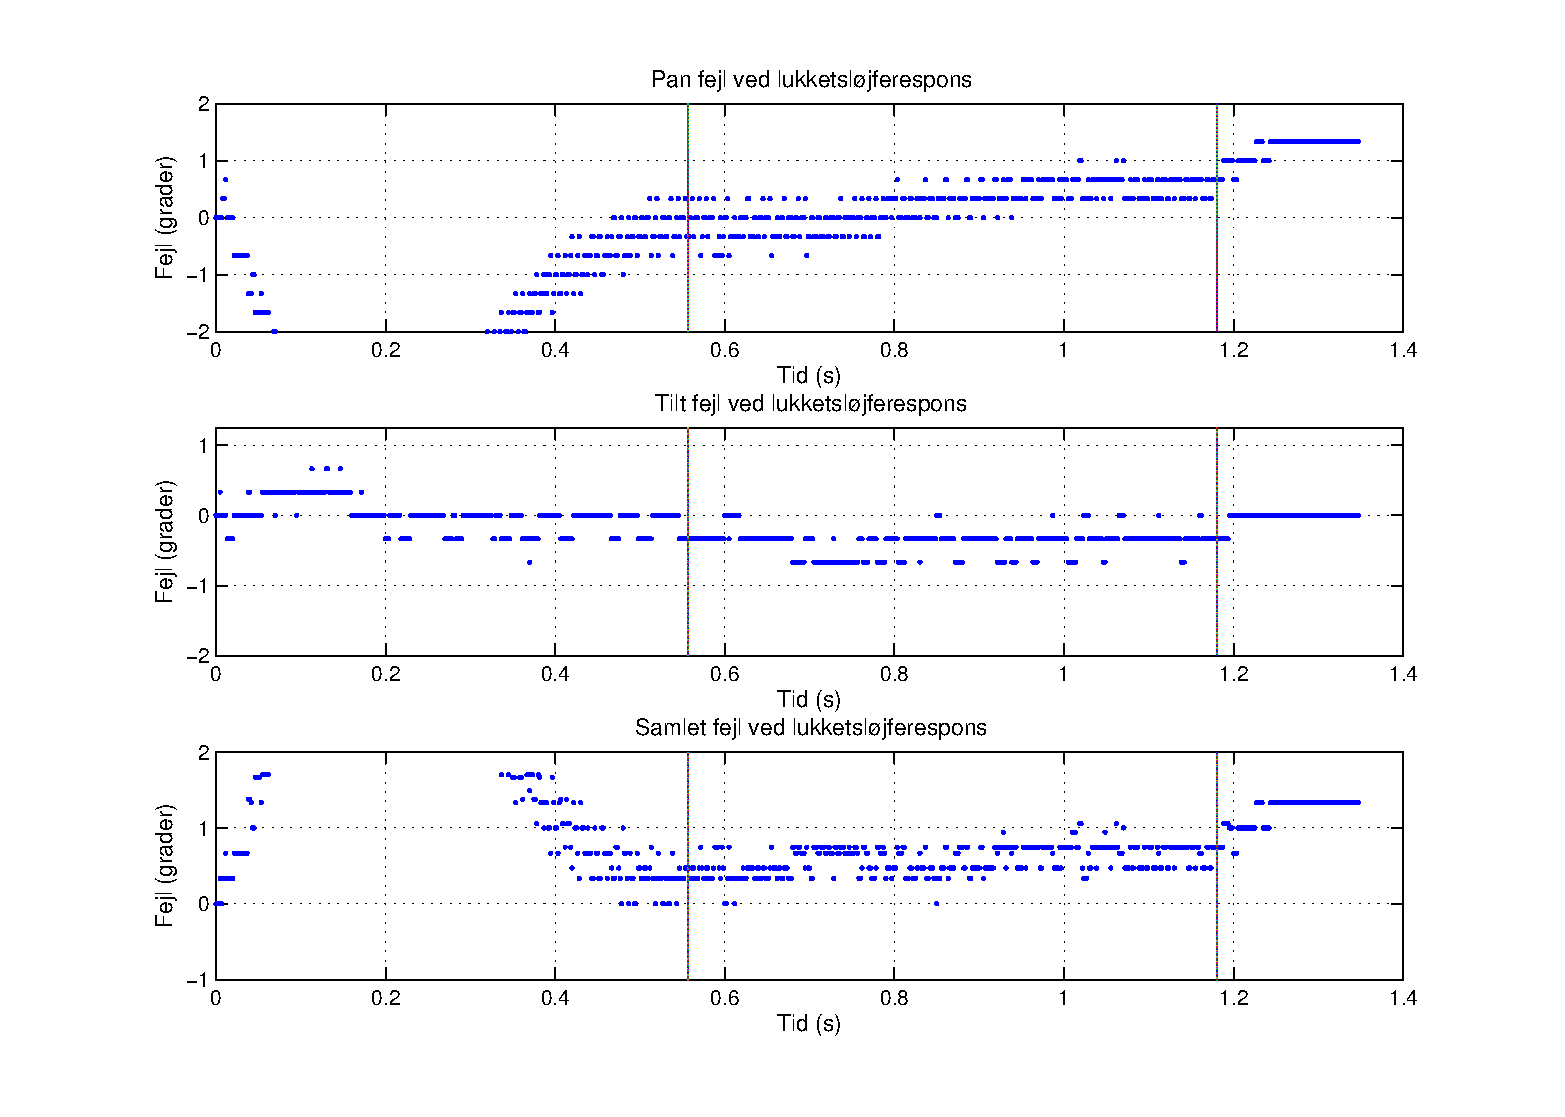
\includegraphics[width=1\textwidth]{./graphics/error_slut.eps}
\caption[Endelig regulator koefficienter]{Tracking fejl målt i grader for hhv. pan og tilt samt den samlet tracking fejl. Testen tager udgangspunkt i koefficienterne fra  tabel \ref{tb:PID_final} og det ses at den samlet tracking fejl opfylder kravet til PTS.} 
\label{fig:PID_final}
\end{figure}

Det viste sig under justeringen at systemet er meget følsomt overfor slid i drivremmene mellem motorerne og Pan- og Tilt-rammerne.
Systemet kræver derfor kalibrering for at kunne fungere i praksis.

\section{Delkonlusion}
Ved Trial-\&-Error-metoden blev regulatorkoefficienterne i Simulink justeret til at give den ønskede 
tracking performance ift. et parabelinput. Pan-koefficienterne giver dårlig performance i praksis.
Ved manuel justering blev et sæt PID-regulatorkoefficienter fundet til Pan, som gav bedre performance.
Det vurderedes nødvendigt at implementere et lavpasfilter til D-leddet.
Med det implementerede filter gav de justerede regulatorkoefficienter en performance,
der ikke ved alle forsøg levede op til kravspecifikationen. Ved nogle af forsøgene viste
systemet sig at leve op til kravene om en Tracking fejl på under 1,02 \degree{} efter 0,557 [s].
Systemet er følsomt overfor slid i drivremmene.
%\include{./content/PTS_verifikation}

\part{Evaluering}
\section{Diskussion}
\label{sec:diskussion}

\todo[inline,author=ALLE]{Mangler at blive skrevet}
\section{Konklusion}
\label{sec:konklusion}
\todo[inline,author=ALLE]{Mangler at blive skrevet}


\subsection{Til viderearbejde}
%%%%%%%%%%%% Litteratur %%%%%%%%%%%%
\bibliography{litteraturliste}
%%%%%%%%%%%% Appendix %%%%%%%%%%%%
\newpage
\appendices
\section{Udregning af tallene}
\label{sec:udregning_af_parabel}
\todo[inline, author=Michael]{Skal sikkert flyttes til appendix?}


Jævnfør reglerne for ES, skal duer/mål passere target crossing point (TCS) som er 
placeret i 4,57 [m] over origo. (0 ; 0 ; 4.57). Fejlmargin for passagen er \(\pm\)0,45 [m]. 
Målene skal desuden flyve 50 - 52 [m].  High house er placeret 20,11 [m] fra TCS, i en 
højde af 3,05 [m]. 

For at simplificere udregningerne, regnes parablen først i 2D. Når denne er fundet kan den tredje dimension tilføjes.  

Da luftmodstanden er negligerbar kan parablen (2. grads polynomium) findes ved at indsætte de kendte punkter. 

Kasteparablen er givet ved vektorfunktionen i ligning  \ref{eq:pf:vektorparabel}.

\begin{equation}
	Pos(t) = \left( \begin{array}{c}
	x_{2D}(t) \\
	y_{2D}(t)
	\end{array}
	\right)
	= \left( \begin{array}{c}
	\cos \theta v_0 t + x_0 \\
	\sin \theta v_0 t - \frac{g}{2} t^2 + y_0
	\end{array}
	\right)
\label{eq:pf:vektorparabel}
\end{equation}

Hvor \(\theta\) er afskydningsvinklen, \(v_0\) er afskydningshastigheden, \(g\) er tyngdeacceleration og \(x_0\), \(y_0\) er begyndelsespunktet. 

For at få en parabel på formen y(x), isoleres t i x(t) med henblik på at substituere t i y(x): (\(x_0\) sættes til 0.)

\begin{equation}
t = \frac{x}{\cos \left( \theta \right) v_0}
\label{eq:pf:x(t)}
\end{equation}

Den fundne værdi for t indsættes i \(y(t)\), og udtrykket reduceres, \citep[Side. 67]{fund_of_physics}: 

\begin{align}
\begin{split}
y(t(x)) &= \sin \left( \theta \right) \frac{x}{\cos \left( \theta \right) v_0} v_0 - \frac{g}{2} \left(\frac{x}{\cos \left( \theta \right) v_0}\right)^2 + y_0 \\
y(x) &= \tan \left( \theta \right) x - \frac{gx^2}{2(\cos \left( \theta \right) v_0)^2} + y_0
\label{eq:pf:y(x(t))}
\end{split}
\end{align}

Det ses at der er 3 ubekendte i ligningen. Dog er 3 punkter kendt fra HH parablen. Det er givet i reglerne for ESS at målet affyres fra en højde på \(y_0\) = 3,05 [m], det indsættes i formlen. 
\begin{equation}
y(x) = \tan \theta x - \frac{gx^2}{2(\cos \left( \theta \right)  v_0)^2} + 3,05
\label{eq:pf:y(x)2}
\end{equation}
Det er givet at målet skal passere TCS som er placeret i en højde på 4,57 [m], 20,11 [m] fra HH. 
Desuden skal målet bevæge sig 50 - 52 [m], i de videre beregninger 52 [m]. Det giver koordinatsættene (20,11 ; 4,57) og (52 ; 0). Vha. disse bestemmes \(\theta\) og \(v_0\) til:\footnote{Ved \(g = 9,82[m/{s}^{2]}\)}
\todo[inline, author=Michael]{Ændre evt. g til 9.816}
\begin{eqnarray}
\theta &=& 9,103 \degree \\
v_0 &=& 34,589 \left[ \frac { m }{ s }  \right] 
\end{eqnarray}

Disse parametre indsættes i vektorfunktionen fra ligning \ref{eq:pf:vektorparabel} samt udtrykket fra ligning \ref{eq:pf:y(x)2}. Udtrykkene reduceres: 

\begin{align}
\begin{split}
	Pos(t) = \left( \begin{array}{c}
	x_{2D}(t) \\
	y_{2D}(t)
	\end{array}
	\right)
	&= \left( \begin{array}{c}
	\cos \left(9,103 \degree \right) 34,589 t \\
	\sin \left(9,103 \degree \right) 34,589 t - \frac{9,82}{2} t^2 + 3,05
	\end{array}
	\right) \\
% ------------------------------
	&= \left( \begin{array}{c}
	34,153 t \\
	- 4,91 t^2 + 5,473 t + 3,05
	\end{array}
	\right)
\label{eq:pf:vektorparabel2}
\end{split}
\end{align}

\begin{align}
\begin{split}
y(x) &= \tan \left(9,103 \degree \right) x - \frac{9,82x^2}{2(\cos \left(9,103 \degree \right) 34,589)^2} + 3,05 \\
% -------------------------------
&= - 0,00421 x^2 + 0,1602 x  + 3,05
\label{eq:pf:y(x)3}
\end{split}
\end{align}

For at finde ud af hvornår målet rammer jorden, sættes \(y(t) = 0\). Det giver:

\begin{equation}
t_{nedslag} = 1,523 [s]
\label{eq:pf:nedslagstid}
\end{equation}

\subsubsection{Parabel i 3 dimensioner}
\label{subsubsec:para}
Nu omskrives parablen fundet i ligning \ref{eq:pf:vektorparabel2} til x,y,z koordinater. 
Grundplanet er XY og højden er givet ved Z. Dvs. at \(z(t) = y_{2D}(t)\) og at \(x(t)\) samt \(y(t)\) afhænger af \(x_{2D}(t)\) samt vinklen \(\alpha\). 
\(\alpha\) er givet ved vinklen mellem parablen projekteret ned på x,y planet (som på figur \ref{fig:para_in_xy_plane}) og y aksen. 
\todo[inline, author=Michael, color=blue! 50]{Kan også skrives som vinklen mellem parablen og x,z planet?}
Vektorfunktionen kan skrives (ved \(\alpha = 15,872 \degree\)): 

\begin{align}
\begin{split}
Pos\left( t \right) = 
\left( \begin{matrix} x\left( t \right)  \\
 y\left( t \right)  \\ 
 z\left( t \right)  \end{matrix} \right) &=
 \left( \begin{matrix} - sin\left( \alpha  \right) \cdot { x }_{ 2D }\left( t \right) + 5.5 \\
 cos\left( \alpha  \right) \cdot { x }_{ 2D }\left( t \right) - 19.3  \\
  { y }_{ 2D }\left( t \right)  \end{matrix} \right)
\\
%----------------------------------------
&= \left( \begin{matrix} - 9,34\cdot t+5,5 \\
  32,851\cdot t-19,3 \\ 
 -{ 4,91\cdot t }^{ 2 }+5,473\cdot t+3,05\end{matrix} \right) 
\label{eq:pf:vektorparabel3d}
\end{split}
\end{align}





Bemærk udgangspunktet for kastet er flyttet fra origo, til HHs position. (Punkt D på figur \ref{fig:para_in_xy_plane})

\newpage
\section{DC motoren}

\subsection{Motorparameter}
\subsection{Eksperiment 1}
\subsubsection{Fremgangsmåde og forsøgsopstilling}
\subsubsection{Databehandling}
Jeg tænker diskussionen kan ligge under databehandlingen. 
\subsubsection{Konklusion}

\subsection{Eksperiment 2}
\subsubsection{Fremgangsmåde og forsøgsopstilling}
\subsubsection{Databehandling}
\subsubsection{Konklusion}


\subsection{Eksperiment 3}
\subsubsection{Fremgangsmåde og forsøgsopstilling}
\subsubsection{Databehandling}
\subsubsection{Konklusion}


\subsection{Eksperiment 4}
\subsubsection{Fremgangsmåde og forsøgsopstilling}
\subsubsection{Databehandling}

\subsubsection{Konklusion}

\subsection{Opsummering af DC motorparameter}
\newpage
\section{Beregning af inertimoment}
\label{sec:inertimomentberegning}
Dette appendix beskæftiger sig med beregningen af de teoretiske inertimomenter
for pan- og tilt-rammerne. Der henvises til figur \ref{fig:inerti_PTS}, og
beregningerne tager udgangspunkt i rammernes mål:
\({L_{1}} =0,292\) [m],
\({L_{2}} =0,280\) [m], \({L_{3}}= 0,42\) [m], \({L_{4}} =0,246\) [m], \({L_{pro}}=0,04\) [m].

\begin{figure}[!th]
\centering
\begin{tikzpicture}[scale=0.7]
\include*{./graphics/inerti_PTS}
\end{tikzpicture}
\caption[Skitse af pan \& tilt-rammerne]{Skitse af pan \& tilt-rammerne.}
\label{fig:inerti_PTS}
\end{figure}

Den teoritiske beregning er foretaget ud fra følgende antagelser og simplificeringer:
\begin{itemize}
\item Aluminimumsprofilen, 40x40L, har en massefylde på \(\rho=1,5\) [kg/m], \citep[Kap. 2 s. 4]{alu_profil_desitet}.
\item Rammerne simplificeres som bestående af tynde stænger, således at hver ramme har to stænger, hvis bidrag
til inertimomentet kan beregnes som var de punktmasser forskudt i forhold til rotationsaksen \citep[s. 254, ligning 10.36]{fund_of_physics},
vha. ligning \ref{eq:punktmasse_para}.
\begin{equation}
J={ J }_{ com }+M\cdot { h }^{ 2 }
\label{eq:punktmasse_para} 
\end{equation}
hvor \({J_{com}} = 0\) og \(h\) er afstand til punktmassen (stangen) fra rotationsaksen.
Inertimomentet for de stænger, der står vinkelret på rotationsakserne, kan beregnes vha. ligning \ref{eq:stang}
\citep[s. 255, tabel 10-2e]{fund_of_physics}.
\begin{equation}
J=\frac { 1 }{ 12 } M\cdot { L }^{ 2 }
\label{eq:stang} 
\end{equation}
\end{itemize}

Med ovenstående formler er det muligt at finde pan og tilt-rammernes teoritiske inertimoment:
\begin{align}
\label{eq:inerti_tilt_pan}
\begin{split}
{ J }_{ tilt,1 } &= \left( \left( 1/12\cdot \rho \cdot { {L_{1}} }^{ 3 } \right) +\left( \rho \left( {L_{2}}-2\cdot {L_{pro}} \right) { \left( \frac { {L_{1}}-{L_{pro}}}{ 2 }  \right)  }^{ 2 } \right)  \right) \cdot 2
\\
 &= 0,0157499 \text{ [kg m$^2$]}
\\
{ J }_{ pan,1 }&=\left( 1/12\cdot \rho \cdot { { L }_{ 3 } }^{ 3 } \right) +\left( \rho \left( { L }_{ 4 }-{ L }_{ pro } \right) { \left( \frac { { L }_{ 3 }-{ L }_{ pro } }{ 2 }  \right)  }^{ 2 } \right) \cdot 2
\\
 &=0,0315708 \text{ [kg m$^2$]}
\end{split}
\end{align}

Tilt-rammens indflydelse på inertimomentet som pan-motoren skal rotere, er afhængig af tilt-rammens vinkel.
Når tilt-rammen er lodret er bidraget til pan-inertimomentet mindst, jf. ligning \ref{eq:punktmasse_para}, fordi afstanden
af to af stængerne til rotationsaksen (pan) er mindst. Ligeledes vil bidraget til pan-inertimomentet være størst når tilt-rammen er vandret.
Dette giver en kobling mellem pan og tilt, hvilket er uønsket under designet af reguleringssløjfen, som beskrevet i afsnit \ref{sec:matPTS}.
En simplificering er således at inkludere bidraget i modellen for pan som en konstant.
Man kan argumentere for, at denne konstant bør være gennemsnittet af bidragene for hele bevægelsen.
Denne ville kunne tilnærmes ud fra den ideelle responskurve for tilt-systemet, der kan beregnes ud fra den faste parabel, som gives som input.
Værdien ville således være baseret på ét specifikt parabelinput. En anden tilgang kunne være at vælge minimum-bidraget, og dermed
have en værdi der er nøjagtig for de tilt-vinkler, der er tæt på lodret, og mere og mere unøjagtig jo mere vandret tilit-vinklen er.
Sidstnævnte tilgang vælges, fordi tilt-vinklen i lerdueskydningen er tilnærmelsesvis lodret. Tilt-rammen roterer i vinkelintervallet \([4,03\degree \leq \phi \leq 12,3\degree]\) jf. lerduens toppunktstid samt nedslagstid på hhv. 0,557 [s] og 1,18 [s], indsat i ligning \ref{eq:sv_koordi}. Antagelsen om konstant bidrag til inertimoment er derfor nøjagtig.

Tilt-rammens bidrag til inertimomentet for pan bestemmes derfor ud fra, at to af tilt-rammens "stænger" er parallele med
rotationsaksen, og at de to stænger med længden \({L_{2}}\) er vinkelret på den, samt at de roterer om den.
Med ligningerne \ref{eq:punktmasse_para} og \ref{eq:stang}
kan tilt-rammens bidrag til pan-inertimomentet altså beregnes vha ligning \ref{eq:tiltOnPan}.
\begin{align}
\begin{split}
J_{pan,tilt_{min}}&=2\cdot{}\left(\frac{1}{12}\cdot{}\rho\cdot{}L_{2}^3
+\rho\cdot{}\left(L_1-2\cdot{}L_{pro}\right)\left(\frac{L_2-L_{pro}}{2}\right)^2\right)
\\
&=0,0146464 \text{ [kg m$^2$]}
\end{split}
\label{eq:tiltOnPan} 
\end{align}
Inertimomentet på pan-aksen er derfor givet ved summationen af pan-rammens inertimoment og tilt-rammens inertimoment,
som angivet i ligning \ref{eq:pan_inerti}.
\begin{align}
\begin{split}
{ J }_{ pan,1.1 } &= J_{ pan,1 }+J_ { pan,tilt_{ min} }
\\
&=0,0462172 \text{ [kg m$^2$]}
\end{split}
\label{eq:pan_inerti} 
\end{align}
Inertimomentet for tilt og pan er beregnet i ligning \ref{eq:inerti_tilt_pan}, mens det endelige inertimomentet for pan er beregnet i ligning \ref{eq:pan_inerti}.
Systemets gearing gør dog at inertimomenterne som motorerne belastes med, er mindre.
Gearingen i EMG30-motoren er i forholdet 30:1, mens gearingen til rammerne er i forholdet 1:3.
Ligning \ref{eq:gearing0} giver forholdet mellem det reflekterede inertimoment \(J_r\) (som motoren belastes med)
og inertimomentet \(J\) efter en gearing med forholdet \(N\) \citep{gear_inerti}.
\begin{equation}
J_r=\frac{J}{N^2}
\label{eq:gearing0}
\end{equation}
\(N\) kan altså bestemmes som multiplikationen af de to gearingsforhold, og er således lig med 10.
I ligning \ref{eq:inerti_tilt_pan_fak} er de reflekterede inertimomenter beregnet.
\begin{align}
\label{eq:inerti_tilt_pan_fak}
\begin{split}
{J_{tilt}}&=1,57499\cdot{10}^{-4} \text{ [kg m$^2$]}
\\
{J_{pan}}&=4,62172\cdot{10}^{-4} \text{ [kg m$^2$]}
\end{split}
\end{align}

\newpage
\section{Serial Peripheral Interface}
\label{app:spi}
Kommunikationen mellem mikrocontolleren og FPGA’en foregår med SPI. 
SPI understøtter full-duplex kommunikation mellem en master og en eller flere slaver.

Der er fire kanaler mellem masteren og slaven: Slave Select (SS), Serial Clock (SCLK), Master Output Slave Input (MOSI) og Master Input Slave Output (MISO). SS bruges til at vælge hvilken slave der skal overføres data til/fra. Den kan også sammenlignes med en chip select. SCLK generes af masteren; SS, MOSI og MISO kører synkront med dette signal.

Opstillingen med en master og en slave kan ses på figur \ref{fig:SPImasterslave}. 
Her kan SS være overflødig, da der kun er en slave at vælge. Til gengæld kan SS bruges til at initialisere overførelsen. 
Når SS er sat højt, begynder overførslen mellem master og slave. Da overførslen er full-duplex sender begge til hinanden samtidig. 
\begin{figure}[!th]
\centering
\begin{tikzpicture}[scale=0.7]
\include*{./graphics/MISOMOSI}
\end{tikzpicture}
\caption[SPI protokol]{Skitse af SPI-kommunikation mellem mikrocontroller og FPGA.}
\label{fig:SPImasterslave}
\end{figure}

Når der er flere slaver, bestemmer SS hvilken slave der overføres til.
Alle slave har deres egen SS, men de deler alle MISO og MOSI. 
Før overførslen begynder sætter masteren SS høj til den ønskede slave,
derefter overføres dataene til slaven.
Mens overførslen finder sted ignorerer de ikke-valgte slaver dataene på MOSI.  
%Det er en standard hvor der bliver overført data mellem en master og en eller flere slaver. 
%Overførelsen sker med full duplex, så der bliver sendt data både fra masteren og slaven på samme tid. 

\begin{figure}[!th]
\centering
\begin{tikzpicture}[scale=0.8]
\include*{./graphics/SPIfigur}
\end{tikzpicture}
\caption[SPI overførelse]{Eksempel på en SPI overførelse.}
\label{fig:SPIfigur}
\end{figure}

Et eksempel på en overførsel mellem en master og en slave kan ses på figur \ref{fig:SPIfigur}. 
Eksemplet tager udgangpunkt i TI Synchronous Serial Frame Format Single Transfer \cite[s. 476]{lm3s6965} fra microcontrolleren.
I denne form er SSIClk, SSIFss, SSITx, SSIRx pins'ne. SSIClk er clock signalet, SSIFss er slave select og SSITx og SSITx er henholdsvis MOSI og MISO.
SCLK har en puls mere, end der er bit i hver data-frame. Det er fordi at SS går høj i den første puls, hvorefter dataene bliver sendt. 
Det gør at SS kan bruges som en indikater for at data vil blive overført.




%%%%%%%%%%%% Bilag %%%%%%%%%%%%
%\part{Bilag}
%%\section{Projektoplæg}
\includepdf[pages={1,2}]{./content/Projekt_2014.pdf}




\end{document} 
